\documentclass[22pt,aspectratio=169]{beamer}

% There are many different themes available for Beamer. A comprehensive
% list with examples is given here:
% http://deic.uab.es/~iblanes/beamer_gallery/index_by_theme.html
% You can uncomment the themes below if you would like to use a different
% one:
%\usetheme{AnnArbor}
%\usetheme{Antibes}
%\usetheme{Bergen}
%\usetheme{Berkeley}
%\usetheme{Berlin}
%\usetheme{Boadilla}
\usetheme{boxes}
%\usetheme{CambridgeUS}
%\usetheme{Copenhagen}
%\usetheme{Darmstadt}
%\usetheme{default}
%\usetheme{Frankfurt}
%\usetheme{Goettingen}
%\usetheme{Hannover}
%\usetheme{Ilmenau}
%\usetheme{JuanLesPins}
%\usetheme{Luebeck}
% \usetheme{Madrid}
%\usetheme{Malmoe}
%\usetheme{Marburg}
%\usetheme{Montpellier}
%\usetheme{PaloAlto}
%\usetheme{Pittsburgh}
%\usetheme{Rochester}
%\usetheme{Singapore}
%\usetheme{Szeged}
% \usetheme{Warsaw}
% \setbeamertemplate{footline}{} % remove footnote line

\usepackage{colortbl}% http://ctan.org/pkg/xcolor
\usepackage[T2A]{fontenc}           % кодировка
\usepackage[utf8]{inputenc}         % кодировка исходного текста
\usepackage[english,russian]{babel}
\hypersetup{unicode=true}
% \usepackage[T1]{fontenc}
\usepackage{mathtools}
\usepackage{listings}
\usepackage{tikz}
\usepackage{tikzpagenodes}
\usetikzlibrary{matrix, patterns, patterns.meta, backgrounds, automata, positioning, tikzmark, calc, arrows, arrows.meta, shapes, shadows.blur, shapes.misc, shapes.callouts}
\usepackage{minted}
\usepackage{advdate}
\usepackage[normalem]{ulem}
\usepackage[export]{adjustbox}
\usepackage{makecell}
\usepackage{environ}
\usepackage{amsmath}
\usepackage{multirow}
\usepackage{pgfplots}
\usepackage{natbib}
\usepackage{bibentry}
\usepackage{nameref}
\usepackage{etoolbox}
\usepackage{hyperref}
\usepackage{pifont} % for ding
\usepackage{subcaption} % for subfigure
\usepackage{appendixnumberbeamer}
\usepackage{diagbox}
\usepackage{stmaryrd}
\setbeamertemplate{blocks}[rounded][shadow=false]

\tikzset{>=latex}
% \font\nullfont=cmr10

\setbeamertemplate{footline}{}
\beamertemplatenavigationsymbolsempty
\setbeamertemplate{footline}[frame number]
\let\otp\titlepage
\renewcommand{\titlepage}{\otp\addtocounter{framenumber}{-1}}


% \BeforeBeginEnvironment{itemize}{\vskip-2ex} % remove spaces before itemize

\newtoggle{fastCompile}
\toggletrue{fastCompile}
\newcommand{\whenFullCompile}[1]{\iftoggle{fastCompile}{
{%\setbeamercolor{background canvas}{bg=red}\begin{frame}{FAST COMPILATION MOCK}\end{frame}
}}{#1}}

\newcommand{\btVFill}{\vskip0pt plus 1fill}


\newcommand\blfootnote[1]{%
  \begingroup
  \renewcommand\thefootnote{}\footnote{#1}%
  \addtocounter{footnote}{-1}%
  \endgroup
}

\tikzset{
    onslide/.code args={<#1>#2}{\only<#1>{\pgfkeysalso{#2}}},
}
\tikzset{/handlers/.provide style/.code={%
    \pgfkeysifdefined{\pgfkeyscurrentpath/.@cmd}{}%
        {\pgfkeys {\pgfkeyscurrentpath /.code=\pgfkeysalso {#1}}}%
}}

\AtBeginDocument{\setlength\abovedisplayskip{0pt}}
% \AtBeginDocument{\setlength\belowdisplayskip{0pt}}

\pgfkeys{%
    /calloutquote/.cd,
    width/.code                   =  {\def\calloutquotewidth{#1}},
    position/.code                =  {\def\calloutquotepos{#1}},
    bubblePosition/.code          =  {\def\calloutquoteBubblePos{#1}},
    author/.code                  =  {\def\calloutquoteauthor{#1}},
    /calloutquote/.unknown/.code   =  {\let\searchname=\pgfkeyscurrentname
                                 \pgfkeysalso{\searchname/.try=#1,
    /tikz/\searchname/.retry=#1},\pgfkeysalso{\searchname/.try=#1,
                                  /pgf/\searchname/.retry=#1}}
                            }

\newcommand\calloutquote[2][]{%
       \pgfkeys{/calloutquote/.cd,
         width               = 5cm,
         position            = {(0,-1)},
         author              = {}}
  \pgfqkeys{/calloutquote}{#1}
  \node [rectangle callout,callout relative pointer={\calloutquotepos},/calloutquote/.cd,
     #1] (tmpcall) at \calloutquoteBubblePos {#2};
  \node at (tmpcall.pointer){\calloutquoteauthor};
}

\newenvironment<>{framesection}[1]{\section{#1}\begin{frame}{#1}#2}{\end{frame}}

\let\oldfootnote\footnote
\renewcommand\footnote[1][]{\oldfootnote[frame,#1]}
\renewcommand{\footref}[1]{\textsuperscript{\ref{#1}}}

\newenvironment<>{varblock}[2][0.9\textwidth]{%
  \begin{center}
    \begin{minipage}{#1}
    \setlength{\textwidth}{#1}%
    \setlength{\linewidth}{\textwidth}% required to itemize respect the width of block
  \begin{actionenv}#3%
    \def\insertblocktitle{#2}%
    \par%
    \usebeamertemplate{block begin}}
  {\par%
  \usebeamertemplate{block end}%
  \end{actionenv}
  \end{minipage}
    \end{center}}



% Variable width example block
\newenvironment<>{varexampleblock}[2][0.9\textwidth]{%
  \begin{center}
    \begin{minipage}{#1}
    \setlength{\textwidth}{#1}%
    \setlength{\linewidth}{\textwidth}%
  \begin{actionenv}#3%
    \def\insertblocktitle{#2}%
    \par%
    \setbeamercolor{local structure}{parent=example text}%
    \usebeamertemplate{block example begin}}
  {\par%
  \usebeamertemplate{block example end}%
    \end{actionenv}
  \end{minipage}
    \end{center}}

% Variable width alert block
\newenvironment<>{varalertblock}[2][0.9\textwidth]{%
  \begin{center}
    \begin{minipage}{#1}
    \setlength{\textwidth}{#1}%
    \setlength{\linewidth}{\textwidth}%
  \begin{actionenv}#3%
    \def\insertblocktitle{#2}%
    \par%
    \setbeamercolor{local structure}{parent=alerted text}%
    \usebeamertemplate{block alerted begin}}
  {\par%
  \usebeamertemplate{block alerted end}%
    \end{actionenv}
  \end{minipage}
    \end{center}}


\tikzset{
    invisible/.style={opacity=0,text opacity=0},
    visible on/.style={alt=#1{}{invisible}},
    alt/.code args={<#1>#2#3}{%
      \alt<#1>{\pgfkeysalso{#2}}{\pgfkeysalso{#3}}
    },
    beameralert/.style={alt=<#1>{fill=red!30,rounded corners}{},anchor=base},
    BeamerAlert/.style={alt=#1{fill=red!30,rounded corners}{},anchor=base}
}
  \newcommand<>{\tikzMe}[1]{% previously: \def\tikzMe<#1>#2{…
    \tikz[baseline]\node[BeamerAlert=#2,anchor=base] {#1};
}

\newcommand{\mattention}[1]{\color{focusColor}#1} % TODO: \bm
\newcommand<>{\mathattention}[1]{\alt#2{\mattention{#1}}{#1}}
% \addtobeamertemplate{block begin}{\setlength\abovedisplayskip{-1cm}}


\newcommand{\currentTableOfContents}{\begin{frame}{Содержание}\tableofcontents[currentsection]\end{frame}}

\newcommand\eqby[1]{\mathrel{\stackrel{\makebox[0pt]{\mbox{\normalfont\tiny #1}}}{=}}}
\newcommand\eqbyref[1]{\mathrel{\stackrel{\makebox[0pt]{\mbox{\normalfont\tiny\eqref{#1}}}}{=}}}
\newcommand\restr[2]{{% we make the whole thing an ordinary symbol
  \left.\kern-\nulldelimiterspace % automatically resize the bar with \right
  #1 % the function
  \vphantom{\big|} % pretend it's a little taller at normal size
  \right|_{#2} % this is the delimiter
  }}

\newcommand{\csharp}{\textsc{C\#}}
\newcommand{\java}{\textsc{Java}}
\newcommand{\scala}{\textsc{Scala}}
\newcommand{\dotnet}{\textsc{.NET}}
\newcommand{\clang}{\textsc{C}}
\newcommand{\cpplang}{\textsc{C++}}
\newcommand{\coq}{\textsc{Coq}}

\lstdefinelanguage{CSharp}
{
 morecomment = [l]{//},
 morecomment = [l]{///},
 morecomment = [s]{/*}{*/},
 morestring=[b]",
 sensitive = true,
 morekeywords = {abstract,  event,  new,  struct,
  as,  explicit,  null,  switch,
  base,  extern,  object,  this,
  bool,  false,  operator,  throw,
  break,  finally,  out,  true,
  byte,  fixed,  override,  try,
  case,  float,  params,  typeof,
  catch,  for,  private,  uint,
  char,  foreach,  protected,  ulong,
  checked,  goto,  public,  unchecked,
  class,  if,  readonly,  unsafe,
  const,  implicit,  ref,  ushort,
  continue,  in,  return,  using,
  decimal,  int,  sbyte,  virtual,
  default,  interface,  sealed,  volatile,
  delegate,  internal,  short,  void,
  do,  is,  sizeof,  while, where,
  double,  lock,  stackalloc,
  else,  long,  static,
  enum,  namespace,  string, Span, var,
  ValueListBuilder}
}

\lstdefinestyle{sharpc}{language=CSharp,
    %frame=lr,
    % frame=l,
    rulecolor=\color{blue!80!black},
    basicstyle=\fontsize{9}{13}\selectfont\ttfamily,
    keywordstyle=\color{blue}\ttfamily,
    stringstyle=\color{red}\ttfamily,
    commentstyle=\color{green}\ttfamily,
    morecomment=[l][\color{magenta}]{\#}
}

\lstdefinelanguage{mycpp}{
  keywords={assume, for, assert},
  keywordstyle=\color{blue}\bfseries,
  keywords=[2]{size_t, int},
  keywordstyle=[2]\color{red}\bfseries,
  identifierstyle=\color{black},
  sensitive=false,
  comment=[l]{//},
  morecomment=[s]{/*}{*/},
  commentstyle=\color{purple}\ttfamily,
  stringstyle=\color{red}\ttfamily,
  morestring=[b]',
  morestring=[b]"
}

\lstset{
   language=mycpp,
   extendedchars=true,
   basicstyle=\small\ttfamily,
   showstringspaces=false,
   showspaces=false,
   tabsize=2,
   breaklines=true,
   showtabs=false
}

\newcommand\eqdef{\mathrel{\stackrel{\makebox[0pt]{\mbox{\normalfont\tiny def}}}{=}}}

\newcommand\drawCodeBox[2]{%
  \begin{tikzpicture}[remember picture,overlay]
    \coordinate (start) at ([yshift=1.7ex]pic cs:#1);
    \coordinate (end) at ([yshift=-0.3ex]pic cs:#2);
    \node[line width=2pt, inner sep=2pt,draw=red,fit=(start) (end)] {};
  \end{tikzpicture}%
}


\newcommand\pair[2]{\langle#1, #2\rangle}
\newcommand\mg[2]{#1=#2}
\newcommand\nmg[2]{#1\neq#2}
\newcommand\li[1]{LI(#1)}
\let\emptyheap\epsilon
\newcommand\agrec{Rec}
\newcommand\agmerge{Merge}
\newcommand\agcompose{\bigcirc}
\newcommand\GRec[1]{\agrec\big(#1\big)}
\newcommand\GMerge[1]{\agmerge\big(#1\big)}
\newcommand\GCompose[2]{#1\agcompose#2}
\newcommand\agho{App}
\newcommand\gapp[1]{\agho(#1)}
\newcommand\GApp[1]{\agho\big(#1\big)}
\newcommand\aunion{union}
\newcommand\union[1]{\aunion\big(#1\big)}
\newcommand\Union[1]{\aunion\Big(#1\Big)}
\newcommand\aderef{read}
\newcommand\afind{find}
\newcommand\find[5]{\afind(#1,#2,#3,#4,#5)}
\newcommand\finD[5]{\afind\big(#1,#2,#3,#4,#5\big)}
\newcommand\Find[5]{\afind\Big(#1,#2,#3,#4,#5\Big)}
\newcommand\deref[2]{\aderef(#1,#2)}
\newcommand\Deref[2]{\aderef\big(#1,#2\big)}
\newcommand\compose[2]{#1\circ#2}
\newcommand\lmbd[2]{\lambda #1.#2}
\newcommand\lmbdx[1]{\lambda x.#1}
\newcommand\dom[1]{dom(#1)}
\newcommand\Dom[1]{dom\big(#1\big)}

\newcommand\exprset{Expr}
\newcommand\guardset{Guard}

\newcommand\pro{\item[$+$]}
\newcommand\contra{\item[$-$]}

\newcommand{\ruquote}[1]{«#1»}

\theoremstyle{plain}
\newtheorem{thm}{Теорема}%[section]
\newtheorem{lem}{Лемма}%[section]
% \newtheorem{crlr}{Corollary}%[section]

\theoremstyle{definition}
\newtheorem{defn}{Определение}
\newtheorem{remk}{Замечание}
\newtheorem{prop}{Утверждение}
\newtheorem{exmp}{Пример}

\newcommand\encircle[1]{%
  \tikz[baseline=(X.base)]
    \node (X) [draw, shape=circle, inner sep=0] {\strut #1};}



\definecolor{dgreen}{rgb}{0.,0.6,0.}
\definecolor{focusGreen}{RGB}{7,225,19}
\definecolor{focusRed}{RGB}{254,31,31}
\definecolor{focusViolet}{RGB}{143,00,255}
\definecolor{focusBlue}{HTML}{1620A6}

\definecolor{myResult}{RGB}{7,225,19}
\definecolor{trivialResult}{RGB}{143,00,255}
\newcommand{\itsMyresult}[1]{\cellcolor{myResult!50}{#1}}
\newcommand{\itsTrivial}[1]{\cellcolor{trivialResult!50}{#1}}

\makeatletter
\pgfdeclarepatternformonly[\LineSpace]{my north east lines}{\pgfqpoint{-1pt}{-1pt}}{\pgfqpoint{\LineSpace}{\LineSpace}}{\pgfqpoint{\LineSpace}{\LineSpace}}%
{
    \pgfsetcolor{\tikz@pattern@color}
    \pgfsetlinewidth{0.4pt}
    \pgfpathmoveto{\pgfqpoint{0pt}{0pt}}
    \pgfpathlineto{\pgfqpoint{\LineSpace + 0.1pt}{\LineSpace + 0.1pt}}
    \pgfusepath{stroke}
}

\pgfdeclarepatternformonly[\LineSpace]{my north west lines}{\pgfqpoint{-1pt}{-1pt}}{\pgfqpoint{\LineSpace}{\LineSpace}}{\pgfqpoint{\LineSpace}{\LineSpace}}%
{
    \pgfsetcolor{\tikz@pattern@color}
    \pgfsetlinewidth{0.4pt}
    \pgfpathmoveto{\pgfqpoint{0pt}{\LineSpace}}
    \pgfpathlineto{\pgfqpoint{\LineSpace + 0.1pt}{-0.1pt}}
    \pgfusepath{stroke}
}
\makeatother

\newdimen\LineSpace
\tikzset{
    line space/.code={\LineSpace=#1},
    line space=7pt
}

\newcommand{\codefontsize}{\footnotesize}

\NewEnviron{onslideenv}{\onslide<2>{\BODY}}{}


\renewcommand{\phi}{\varphi}

\newcommand{\pdr}{IC3/PDR}
\newcommand{\cegar}{CEGAR}
\newcommand{\ice}{ICE}
\newcommand{\fmf}{FMF}
\newcommand{\satur}{Насыщение}

\newcommand{\theregclass}{Reg}
\newcommand{\regclass}{\textsc{\theregclass{}}}
\newcommand{\theelemclass}{Elem}
\newcommand{\elemclass}{\textsc{\theelemclass{}}}
\newcommand{\elemextclass}{\textsc{\theelemclass{}\textsubscript{*}}}
\newcommand{\sizeelemclass}{\textsc{Size\theelemclass{}}}
\newcommand{\sizeelemextclass}{\textsc{Size\theelemclass{}\textsubscript{*}}}
\newcommand{\catelemclass}{\textsc{Cat\theelemclass{}}}
\newcommand{\syncRegFlatClass}{\regclass{}\textsubscript{+}} %TODO: take it from Haudebourg
\newcommand{\syncRegFullClass}{\regclass{}\textsubscript{$\times$}}
\newcommand{\regelemclass}{\textsc{\theelemclass{}\theregclass{}}}

\newcommand{\zprover}{\textsc{Z3}}
\newcommand{\cvc}{\textsc{cvc5}}
\newcommand{\princess}{\textsc{Princess}}
\newcommand{\chaff}{\textsc{Chaff}}
\newcommand{\cvcind}{\textsc{\cvc{}-Ind}}
\newcommand{\mace}{\textsc{Mace4}}
\newcommand{\kodkod}{\textsc{Kodkod}}
\newcommand{\paradox}{\textsc{Paradox}}
\newcommand{\vampire}{\textsc{Vampire}}
\newcommand{\eprover}{\textsc{E}}
\newcommand{\zipperposition}{\textsc{Zipperposition}}

\newcommand{\eldarica}{\textsc{Eldarica}}
\newcommand{\theringen}{\textsc{RInGen}}
\newcommand{\ringenAny}[2]{#1(#2)}
\newcommand{\ringenSyncAny}[1]{\textsc{#1-Sync}}
\newcommand{\theringenCICIAny}[1]{\textsc{#1-CICI}}
\newcommand{\ringenCICIAny}[2]{\theringenCICIAny{#1}(#2)}
\newcommand{\ringen}[1]{\ringenAny{\theringen}{#1}}
\newcommand{\ringenSync}{\ringenSyncAny{\theringen}}
\newcommand{\theringenCICI}{\theringenCICIAny{\theringen}}
\newcommand{\ringenCICI}[1]{\ringenCICIAny{\theringen}{#1}}
\newcommand{\verifier}{\mathcal{V}}
\newcommand{\spacer}{\textsc{Spacer}}
\newcommand{\racer}{\textsc{Racer}}
\newcommand{\hoice}{\textsc{HoIce}}
\newcommand{\rchc}{\textsc{RCHC}}
\newcommand{\vericat}{\textsc{VeriCaT}}
\newcommand{\verimap}{\textsc{VeriMAP-iddt}}

\newcommand{\signature}{\Sigma}
\newcommand{\theory}{\mathcal{T}}
\newcommand{\relations}{\mathcal{R}}
\newcommand{\oracle}{\mathcal{O}}
\newcommand{\ourCEGAR}{\cegar{}($\oracle$)}
\newcommand{\prog}{\mathcal{S}}
\newcommand{\fsymbs}{\signature_F}
\newcommand{\btuple}[1]{\big\langle #1 \big\rangle}
\newcommand{\theautomaton}[4]{\btuple{#1, #2, #3, #4}}
\newcommand{\autInit}{s_0}
\newcommand{\autStates}{S}
\newcommand{\autFinStates}{\autStates_F}
\newcommand{\autTrans}{\Delta}
\newcommand{\autApp}[1]{A\left(#1\right)}
\newcommand{\automaton}[3]{\theautomaton{#1}{\fsymbs}{#2}{#3}}
\newcommand{\automatonDef}{\automaton{\autStates}{\autFinStates}{\autTrans}}
\newcommand{\Automaton}[2]{\automaton{\{#1\}}{\{#2\}}{\autTrans}}
\newcommand{\sautomatonGen}[4]{\theautomaton{#1}{\fsymbs^{\leq #2}}{#3}{#4}}
\newcommand{\sautomaton}[3]{\sautomatonGen{\{#1\}}{#2}{\{#3\}}{\autTrans}}


\newcommand{\structur}{\mathcal{H}}
\newcommand{\mystructur}{\mathcal{M}}
\newcommand{\invariant}{\mathcal{I}}
\newcommand{\thedomain}{\left|\mystructur\right|}
\newcommand{\domain}[1]{\thedomain_{#1}}
\newcommand{\tuple}[1]{\langle #1 \rangle}


\let\oldemptyset\emptyset
\let\emptyset\varnothing

\newcommand{\formallang}{\mathbf{L}}
\newcommand{\automat}{\mathcal{A}}
\newcommand{\langOf}[1]{\mathcal{L}(#1)}
\newcommand{\height}[1]{\mathcal{H}eight(#1)}

\definecolor{badInvariantColor}{RGB}{255,50,50}
\definecolor{goodInvariantColor}{RGB}{5,150,2}
\definecolor{darkyellow}{RGB}{153,153,0}
\definecolor{focusColor}{RGB}{230,5,5}
\definecolor{nicegreen}{RGB}{5,150,2}
% \definecolor{nicegreen}{rgb}{0.0, 0.8, 0.3}
\newcommand{\xmark}{\text{\ding{53}}}%

\newcommand{\attention}[1]{\textcolor{badInvariantColor}{\textbf{#1}}}

\makeatletter
\newcommand*{\currentname}{\@currentlabelname}
\makeatother

\newcommand{\beamermessage}[2]{%
\begin{beamercolorbox}[wd=#1,center,rounded=true]{author in head/foot}
#2
%[wd=#1,ht=3ex,dp=2ex,center,rounded=true]{author in head/foot}
%\hfill\parbox[c][7ex][c]{#1}{\centering\LARGE #2}\hfill\null
\end{beamercolorbox}}

\makeatletter
\newcommand*\Alt{\alt{\Alt@branch0}{\Alt@branch1}}

\newcommand\Alt@branch[3]{%
  \begingroup
  \ifbool{mmode}{%
    \mathchoice{%
      \Alt@math#1{\displaystyle}{#2}{#3}%
    }{%
      \Alt@math#1{\textstyle}{#2}{#3}%
    }{%
      \Alt@math#1{\scriptstyle}{#2}{#3}%
    }{%
      \Alt@math#1{\scriptscriptstyle}{#2}{#3}%
    }%
  }{%
    \sbox0{#2}%
    \sbox1{#3}%
    \Alt@typeset#1%
  }%
  \endgroup
}

\newcommand\Alt@math[4]{%
  \sbox0{$#2{#3}\m@th$}%
  \sbox1{$#2{#4}\m@th$}%
  \Alt@typeset#1%
}

\newcommand\Alt@typeset[1]{%
  \ifnumcomp{\wd0}{>}{\wd1}{%
    \def\setwider   ##1##2{##2##1##2 0}%
    \def\setnarrower##1##2{##2##1##2 1}%
  }{%
    \def\setwider   ##1##2{##2##1##2 1}%
    \def\setnarrower##1##2{##2##1##2 0}%
  }%
  \sbox2{}%
  \sbox3{}%
  \setwider2{\wd}%
  \setwider2{\ht}%
  \setwider2{\dp}%
  \setnarrower3{\ht}%
  \setnarrower3{\dp}%
  \leavevmode
  \rlap{\usebox#1}%
  \usebox2%
  \usebox3%
}
\makeatother

\newcommand{\Focus}[2]{{\begin{center}#1 #2\end{center}}}
\newcommand{\focus}[1]{\Focus{\huge}{#1}}

% \DeclareFieldFormat*{citetitle}{<<#1>>} % removes ``quotes'' from title
% \newcommand{\citee}[1]{\citetitle{#1}}
\newcommand{\citee}[1]{\bibentry{#1}}

\newcommand{\chccomp}{CHC-COMP}
\newcommand{\fsharp}{F\#}

\delimitershortfall=-1pt % вложенные скобки

\newcolumntype{x}[1]{>{\centering\let\newline\\\arraybackslash\hspace{0pt}}p{#1}}
\newcommand{\tnote}[1]{$^{#1}$}
\newcommand{\exRef}[1]{\textit{#1}}
\newcommand{\exEvenLeft}{\exRef{even}}
\newcommand{\exLR}{\exRef{lr}}
\newcommand{\exLt}{\exRef{lt}}
\newcommand{\exNode}{\exRef{node}}
\title{Автоматический вывод индуктивных инвариантов программ с алгебраическими типами данных}
\titlegraphic{\includegraphics[height=.1\textheight]{resources/block_ru.pdf}}

\author{Костюков Юрий Олегович}
% {\footnotesize\textcolor{gray}{группа 571\\научный руководитель: cт. преп. Д.\,А. Мордвинов}}

% - Give the names in the same order as the appear in the paper.
% - Use the \inst{?} command only if the authors have different
%   affiliation.

\institute[] % (optional, but mostly needed)
{
    Научный руководитель:\\д.\:т.\:н., доцент Кознов Дмитрий Владимирович
    % Санкт-Петербургский государственный университет
}
% - Use the \inst command only if there are several affiliations.
% - Keep it simple, no one is interested in your street address.

% \day=15
% \month=12
% \year=2023

% \date{\today}
\date{2023}

\begin{document}

% \toggletrue{fastCompile}
\togglefalse{fastCompile}

\newcommand\exprVsAutomationPlot{
\begin{tikzpicture}[domain=0:4]
    \draw[->] (-0.5,0) -- (7,0) node[below] {Возможность автоматизации};
    \draw[->] (0,-0.5) -- (0,5) node[above] {Выразительность};
    \draw (2,4) node [circle,fill,inner sep=1pt,label=above:\textsc{Coq}-термы] {};
    \draw (5,2.5) node [circle,fill,inner sep=1pt,label=above:\emph{Новое представление}] {};
    \draw (5,1.25) node [circle,fill,inner sep=1pt,label=above:FOL-формулы] {};
    % \draw[color=red] plot[id=x] function{x} 
    %     node[right] {$f(x) =x$};
    % \draw[color=blue] plot[id=sin] function{sin(x)} 
    %     node[right] {$f(x) = \sin x$};
    % \draw[color=orange] plot[id=exp] function{0.05*exp(x)} 
    %     node[right] {$f(x) = \frac{1}{20} \mathrm e^x$};
\end{tikzpicture}
}

\newcommand{\ciciPic}{
\tikzset{empty block/.style={minimum width=70pt,minimum height=30pt}}
\tikzset{block/.provide style={empty block, draw, rounded rectangle}}
\hspace*{-5mm}
\begin{tikzpicture}[every node/.style={align=center,font=\small}]

% \begin{scope}[overlay]
% \draw[line width=3,onslide=<3->{dash pattern={on 10pt off 10pt}}] (14, -3) circle (240pt);
% \node[rotate=-10] at (-2, -4.5) {\Large\textbf{Хорн-решатели}};
% \node[rotate=10] at (8, -4.5) {\Large\textbf{Инструменты}\\\textbf{вывода теорем}};
% \end{scope}

% \only<1>{
% \begin{scope}[overlay,node distance=30pt]
% \node (z3) at (0,-1) {\textsc{Z3/Spacer}};
% \node[below left=of z3] {\textsc{Eldarica}};
% \node[below right=of z3] {\textsc{Hoice}};
% \node[below=of z3] {\textsc{Golem}};
% \node[above left=of z3] {\textsc{FreqHorn}};
% \node[above right=of z3] {\textsc{QARMC}};
% \node[above=of z3] {\textsc{Duality}};
% \end{scope}}

% \only<1-2>{
% \begin{scope}[overlay,node distance=20pt]
% \node (vampire) at (8,-1) {\textsc{Vampire}};
% \node[right=of vampire] {\textsc{E}};
% \node[below=of vampire] {\textsc{Zipperposition}};
% \node[above=of vampire] {\textsc{iProver}};
% \node[above right=of vampire] {\textsc{cvc5}};
% % \node[above right=of vampire] {\textsc{QARMC}};
% % \node[above=of vampire] {\textsc{Duality}};
% \end{scope}
% }

% \uncover<2->{
\begin{scope}[node distance=50pt]
\node[block] (isFeasible) {\textsc{IsFeasible}};
\node[block,below=of isFeasible] (modelCheck) {\textsc{Validate}};
\node[block,right=of modelCheck] (refine) {\textsc{Refine}};
\node[left=of isFeasible] (unsafe) {UNSAT};
\node[left=of modelCheck] (safe) {SAT};
\draw[->] (isFeasible) -- (unsafe) node [midway,above] {трасса};
\draw[->] (modelCheck) -- (safe) node [midway] {инд.\\инвариант};
\draw[->] (refine) -- (modelCheck);
\draw[->] (modelCheck) -- (isFeasible) node [midway,left=-1mm,align=right] {абстрактная\\трасса};

\uncover<2->{
\node[block,above=of refine] (runOracle) {\textsc{Collaborate}};
\path (runOracle) -- (refine) node [midway] (tmp) {};
\node[block,right=108pt of tmp] (atp) {Инструмент\\вывода\\теорем};
\draw[->] (isFeasible) -- (runOracle);
\draw[->] (runOracle) -- (atp) node [pos=.65,sloped] {\textit{остаточная}\\\textit{система}};
\draw[->] (atp) -- (refine) node [pos=.4,sloped] {\textcolor{focusRed}{абстр. трасса}\\\textcolor{focusGreen}{част. инвариант}};
% \only<4>{
\calloutquote[width=30mm,textwidth=30mm,position={(0.7,0.1)},bubblePosition={(3,-1.5)},callout pointer width=.4cm,fill=yellow!80,rounded corners]{Её достижимые состояния~--- это\\состояния исходной без состояний\\текущего кандидата в инварианты}
% }
}
\only<1>{
\node (runOracle) [empty block,above=of refine] {};
\draw (isFeasible) -- (runOracle.center);
\draw[->] (runOracle.center) -- (refine);
}
\end{scope}
% }



% \onslide<3>{\filldraw [line width=3,fill opacity=0.4,fill={rgb, 255:red, 7; green, 225; blue, 19 }] (-7.5, 2) circle (300pt);}

% \onslide<4>{
% % print(''.join(["\\textcolor{focus%s}{\\textsc{%s}}" % ("Red" if i % 2 else "Green", x) for i,x in enumerate(a)]))
% \node[draw=focusRed,dash pattern={on 7pt off 9pt},postaction={draw=focusGreen, dash phase=8pt},align=center,inner sep=5mm,line width=2.75pt] at (500,320) {\LARGE \textcolor{focusGreen}{\textsc{C}}\textcolor{focusRed}{\textsc{o}}\textcolor{focusGreen}{\textsc{l}}\textcolor{focusRed}{\textsc{l}}\textcolor{focusGreen}{\textsc{a}}\textcolor{focusRed}{\textsc{b}}\textcolor{focusGreen}{\textsc{o}}\textcolor{focusRed}{\textsc{r}}\textcolor{focusGreen}{\textsc{a}}\textcolor{focusRed}{\textsc{t}}\textcolor{focusGreen}{\textsc{i}}\textcolor{focusRed}{\textsc{o}}\textcolor{focusGreen}{\textsc{n}}};}
\end{tikzpicture}}

\newcommand{\toolplotTwo}[2]{%
% #1 is backend solver name
% #2 is a .csv file name
\pgfplotstableread[col sep = comma]{#2}\toolplotcsv
\begin{subfigure}[t]{0.47\textwidth}
\begin{center}
\begin{tikzpicture}[scale=.55]
\begin{axis}[xmode=log, ymode=log, legend pos= north west, xlabel={\ringenCICI{#1}, мс}, ylabel style = {align=center}, ylabel={{\color{red}\racer{}} и {\color{blue}\ringen{#1}}, мс}]
    \addplot[dashed,no marks,very thin] coordinates {(10,10) (1200000,1200000)};
    \addplot [dashed, no marks, thin] coordinates {(10,10) (1200000,1200000)};
    \addplot [dashed, no marks, thin] coordinates {(10,600000) (600000,600000)};
    \addplot [dashed, no marks, thin] coordinates {(600000, 10) (600000,600000)};
    \addplot [dashed, no marks, thin] coordinates {(10, 1200000) (1200000,1200000)};
    \addplot [dashed, no marks, thin] coordinates {(1200000, 10) (1200000,1200000)};
    
    % one second
    \addplot [no marks, thin] coordinates {(1000, 10) (1000,1000)};
    \addplot [no marks, thin] coordinates {(10, 1000) (1000,1000)};

    \addplot  [only marks,  mark=o, color=red,  mark size=3pt] table [x={Collab}, y={Z3}] {\toolplotcsv};
    \addplot  [only marks,  mark=triangle, color=blue, mark size=3pt] table [x={Collab}, y={RInGen}] {\toolplotcsv};
\end{axis}
\end{tikzpicture}
\end{center}
\end{subfigure}
}

\newcommand{\residualPic}{
\tikzset{
    importantNode/.style={font=\Large},
    test1/.style={diamond, aspect=2, text width=5em, inner sep=5pt}}
\begin{tikzpicture}
\def\Bad{(9, 1.0) ellipse[x radius=15mm, y radius=15mm]}
\def\Abstrk{(-1.5, -2.1) rectangle ++(4.6, 4.2)}
\def\Abstr{(-2.2, -2.7) rectangle ++(10.5, 5.4)}
\def\TAbstrk{(-1.2, 0) -- (-0.8,0.8) -- (1,1.5) -- (4,1) -- (5,0) -- (4,-1) -- (1,-1.5) -- (-0.8,-0.8) -- cycle}
\def\Reach{(2.7,0) ellipse [x radius=40mm, y radius=20mm]}
\def\ReachRes{(2.8,-2.2) rectangle ++(4.2, 4.4)}
\def\OracleInv{(4.9,0) ellipse [x radius=26mm, y radius=40mm]}
\def\AroundOracleInv{(4.9,0) ellipse [x radius=76mm, y radius=41mm]}


\uncover<1-7>{
\draw (0,0) ellipse [x radius=10mm, y radius=5mm] node (init) {$Init=R_0$};
}

\draw[draw=focusRed,ultra thick] \Bad node[importantNode] {\textcolor{focusRed}{$Bad$}};

\uncover<2-7>{
\draw (0.9,0) ellipse [x radius=20mm, y radius=10mm] node {};
\node[right=3mm of init.east] (dots) {$\ldots$};
\node[right=3mm of dots] (rk) {$R_k$};
}


\uncover<3-8, 13->{\draw[thick] \Reach;}
\uncover<3-11, 13->{\node[importantNode,right=31mm of rk] (justr) {$R_{\invisible{k}}$};}
\uncover<3-11>{\node[left=3mm of justr] (dots2) {$\ldots$};}

\uncover<4>{\draw[overlay,ultra thick] (5, 5) -- (9.5, -5);}


\uncover<6-12>{
\uncover<3-8>{\draw \TAbstrk;}
\alt<8->{
    \node [importantNode,left=5mm of dots2] (tak) {$Init'$};
}{
    \node [importantNode,left=2mm of dots2] (tak) {$T(A_k)$};
}
\begin{scope}
\uncover<9-12>{
  \clip \TAbstrk;
  \draw[thick,focusGreen] \Abstrk;
}
\end{scope}
\begin{scope}
\uncover<9-11>{
  \clip \Reach;
  \draw[thick] \Abstrk;
}
\end{scope}
\begin{scope}[even odd rule]
\uncover<9-12>{
  \clip \Abstrk \Abstr;
  \uncover<-11>{\draw[thick] \Reach;}
  \draw[thick,focusGreen] \TAbstrk;
}
\end{scope}
\begin{scope}[even odd rule]
\uncover<9-12>{
  \clip \Abstrk \Abstr;
  \fill[pattern={Lines[angle=45,distance=4pt,line width=0.3mm]},pattern color=focusGreen] \TAbstrk;
}
\end{scope}
}

\uncover<10-12>{
  \draw[thick,focusGreen] \ReachRes;
  \node[importantNode] (Rres) at (5.8, 1.9) {\textcolor{focusGreen}{$R'$}};
  \path[initial/.tip = {latex},-initial] (tak) edge [bend right,thick,focusGreen] node[black,importantNode,left=-1mm] {$T'^*$} (Rres);
}

\uncover<12>{
  \draw[ultra thick,focusBlue] \OracleInv;
}
\uncover<13->{
  \fill[pattern={Lines[angle=45,distance=4pt,line width=0.3mm]},pattern color=focusBlue] \OracleInv;
  \begin{scope}[overlay,even odd rule]
  \clip \Abstrk \AroundOracleInv;
  \draw[ultra thick,focusBlue] \OracleInv;
  \end{scope}
}
\uncover<12->{\node[importantNode] at (2.9, 3.2) {\textcolor{focusBlue}{$B$}};}

\begin{scope}[overlay,even odd rule]
\uncover<13->{
  \clip \OracleInv \AroundOracleInv;
  \draw[draw=focusViolet,ultra thick] \Abstrk;
  % \fill[pattern=my north west lines,pattern color=focusViolet] \Abstrk;
  % \fill[overlay,pattern=my north west lines,pattern color=focusViolet] \Abstrk;
  % \fill[pattern=north west lines,pattern color=focusViolet] \Abstrk;
  \fill[pattern={Lines[angle=-45,distance=4pt,line width=0.3mm]},pattern color=focusViolet] \Abstrk;
}
\end{scope}

\uncover<5-8>{
\draw[draw=focusViolet,ultra thick,onslide=<8>{fill=white}] \Abstrk;
\node (ak) at (3, -1.1) {};
}
\uncover<5-8,13->{\node[importantNode] at (-1, 2.4) {\textcolor{focusViolet}{$A_k$}};}

\uncover<6-7>{\path[initial/.tip = {latex},-initial] (ak) edge [bend right,thick] (tak);}
\uncover<7>{
\draw[draw=focusViolet,ultra thick] \Abstr;
\node[importantNode] (akp1) at (7.8, -1.1) {\textcolor{focusViolet}{$A_{k+1}$}};
\path[initial/.tip = {latex},-initial] (tak) edge [bend right,thick,focusViolet] (akp1);
\begin{scope}
\uncover<7>{
  \clip \Abstr;
  \fill[pattern={Lines[angle=45,distance=4pt,line width=0.3mm]},pattern color=focusViolet] \Bad;
}
\end{scope}}

\begin{scope}[overlay,font=\Large]
\only<-4>{\node[font=\large] at (-1.5,3) {
    \begin{minipage}{40mm}
    \begin{align*}
    Init(x) &\rightarrow I(x)\\
    I(x) \land Tr(x, x') &\rightarrow I(x')\\
    I(x) \land Bad(x) &\rightarrow \bot
    \end{align*}
    \end{minipage}
};}
\node at (4, -3.4) {\begin{minipage}{\textwidth}
\only<2>{$$R_{k}(x) = R_{k-1}(x) \lor \exists x'. \big(R_{k-1}\left(x'\right) \land Tr\left(x', x\right)\big)$$}
\only<3>{$$R(x) = \bigvee_{k=0}^\infty R_{k}(x)$$}
\only<4>{$$\models \forall x. \big(R(x) \land Bad(x) \rightarrow \bot\big)$$}
\only<5>{\centering for each $i$, $\models R_i(x) \rightarrow A_i(x)$}
\only<6>{$$\text{transition }T(A)(x) = \exists x'. \big(A(x') \land Tr(x', x)\big)$$}
\only<7>{$$A_{k+1} = \alpha\big(T(A_k)\big)\text{ for abstraction }\alpha$$}
\only<8-9>{\large $$Init' \text{ of residual system is } T(A_k)\Alt<8>{\land\neg}{\ \setminus} A_k\text{~--- \textbf{one-step non-inductive states}}$$}
\only<10>{$$\text{transition }T'(B)\text{ of residual system is } T(B)\setminus A_k$$}
\only<11>{\large $$R' = \text{reachable in residual system}=\text{reachable from non-inductive subset of }A_k$$}
\end{minipage}};
\only<7>{\calloutquote[position={(2,-1.9)},bubblePosition={(5.5,3.3)},callout pointer width=.5cm,fill=focusViolet!50,rounded corners]{abstract counterexample}}
\only<12>{\calloutquote[position={(1.77,-1.9)},bubblePosition={(-0.75,2)},callout pointer width=.6cm,fill=focusBlue!50,rounded corners,font=\large]{\begin{minipage}{45mm}
% $B$~-- residual system invariant obtained from oracle:
\begin{align*}
B \text{ -- } &\text{residual system invariant}\\
&\text{obtained from oracle:}
\end{align*}\vspace*{-8mm}
% \alt<13>{\begin{align*}
%     A_k(x') \land Tr(x', x) \land \neg A_k(x) &\rightarrow B(x)\\
%     B(x) \land Tr(x, x') \land \neg A_k(x') &\rightarrow B(x')\\
%     B(x) \land Bad(x) &\rightarrow \bot
% \end{align*}}{
\begin{align*}
    Init'(x) &\rightarrow B(x)\\
    B(x) \land Tr'(x, x') &\rightarrow B(x')\\
    B(x) \land Bad(x) &\rightarrow \bot
    \end{align*}
    % }
\end{minipage}}}
\only<14>{\node[draw,fill=focusViolet!40,opacity=0.95,rounded rectangle,minimum height=2cm,rotate=0,align=center] at (4,-2) {\begin{minipage}{.85\textwidth}
\centering $A_k \lor B$~--- \textbf{combined invariant} of the original system:
\begin{align*}
R(x) &\rightarrow A_k(x)\lor B(x)\\
\big(A_k(x)\lor B(x)\big) \land Bad(x) &\rightarrow \bot
\end{align*}
\end{minipage}};}
\end{scope}
\end{tikzpicture}
}

% %Rounded Rect [id:dp9443796803339821] 
% \draw   (170,249) .. controls (170,244.58) and (173.58,241) .. (178,241) -- (272,241) .. controls (276.42,241) and (280,244.58) .. (280,249) -- (280,273) .. controls (280,277.42) and (276.42,281) .. (272,281) -- (178,281) .. controls (173.58,281) and (170,277.42) .. (170,273) -- cycle ;
% %Rounded Rect [id:dp2773818458647491] 
% \draw   (170,148) .. controls (170,143.58) and (173.58,140) .. (178,140) -- (262,140) .. controls (266.42,140) and (270,143.58) .. (270,148) -- (270,172) .. controls (270,176.42) and (266.42,180) .. (262,180) -- (178,180) .. controls (173.58,180) and (170,176.42) .. (170,172) -- cycle ;
% % Refine rect
% \draw   (380,248) .. controls (380,243.58) and (383.58,240) .. (388,240) -- (472,240) .. controls (476.42,240) and (480,243.58) .. (480,248) -- (480,272) .. controls (480,276.42) and (476.42,280) .. (472,280) -- (388,280) .. controls (383.58,280) and (380,276.42) .. (380,272) -- cycle ;
% %Straight Lines [id:da932730372325787] 
% \draw    (380,261) -- (283,261) ;
% \draw [shift={(280,261)}, rotate = 360] [fill={rgb, 255:red, 0; green, 0; blue, 0 }  ][line width=0.08]  [draw opacity=0] (8.93,-4.29) -- (0,0) -- (8.93,4.29) -- cycle    ;
% %Straight Lines [id:da4961993079694478] 
% \draw    (220,240) -- (220,183) ;
% \draw [shift={(220,180)}, rotate = 90] [fill={rgb, 255:red, 0; green, 0; blue, 0 }  ][line width=0.08]  [draw opacity=0] (8.93,-4.29) -- (0,0) -- (8.93,4.29) -- cycle    ;
% %Straight Lines [id:da36870516429389966] 
% \draw    (170,260) -- (93,260) ;
% \draw [shift={(90,260)}, rotate = 360] [fill={rgb, 255:red, 0; green, 0; blue, 0 }  ][line width=0.08]  [draw opacity=0] (8.93,-4.29) -- (0,0) -- (8.93,4.29) -- cycle    ;
% %Straight Lines [id:da24013791401632556] 
% \draw    (170,160) -- (93,160) ;
% \draw [shift={(90,160)}, rotate = 360] [fill={rgb, 255:red, 0; green, 0; blue, 0 }  ][line width=0.08]  [draw opacity=0] (8.93,-4.29) -- (0,0) -- (8.93,4.29) -- cycle    ;



% \onslide<2->{
% %Rounded Rect [id:dp3414133323513948] 
% \draw   (380,148) .. controls (380,143.58) and (383.58,140) .. (388,140) -- (472,140) .. controls (476.42,140) and (480,143.58) .. (480,148) -- (480,172) .. controls (480,176.42) and (476.42,180) .. (472,180) -- (388,180) .. controls (383.58,180) and (380,176.42) .. (380,172) -- cycle ;
% %Straight Lines [id:da3745745784791844] 
% % Right Arrows
% \draw    (270,160) -- (377,160) ;
% \draw    (430,180) -- (430,237) ;
% \draw [shift={(380,160)}, rotate = 180] [fill={rgb, 255:red, 0; green, 0; blue, 0 }  ][line width=0.08]  [draw opacity=0] (8.93,-4.29) -- (0,0) -- (8.93,4.29) -- cycle    ;
% % Text Node
% \draw (370,197) node [anchor=north west][inner sep=0.75pt]   [align=center] {abstract\\cex};
% % Text Node
% \draw (379,150) node [anchor=north west][inner sep=0.75pt]   [align=center] {\textsc{RunOracle}};


% % Text Node
% \draw (588,160) node [anchor=north west][inner sep=0.75pt]  [align=center] {Black-Box Solver};
% %Rounded Rect [id:dp2146350233524532] 
% \draw   (580,152) .. controls (580,145.37) and (585.37,140) .. (592,140) -- (698,140) .. controls (704.63,140) and (710,145.37) .. (710,152) -- (710,188) .. controls (710,194.63) and (704.63,200) .. (698,200) -- (592,200) .. controls (585.37,200) and (580,194.63) .. (580,188) -- cycle ;

% \alt<4->{
% % predicates arrow
% \draw    (480,160) -- (577.13,170) ;
% \draw [shift={(580,170)}, rotate = 186.7] [fill={rgb, 255:red, 0; green, 0; blue, 0 }  ][line width=0.08]  [draw opacity=0] (8.93,-4.29) -- (0,0) -- (8.93,4.29) -- cycle    ;
% % abs cex arrow
% \draw    (600,200) -- (480,259.28) ;
% \draw [shift={(480,259)}, rotate = 336.17] [fill={rgb, 255:red, 0; green, 0; blue, 0 }  ][line width=0.08]  [draw opacity=0] (8.93,-4.29) -- (0,0) -- (8.93,4.29) -- cycle    ;
% % Text Node
% \draw (492,139) node [anchor=north west][inner sep=0.75pt]  [rotate=-6.23] [align=center] {\textcolor{focusGreen}{\textbf{predicates}}};
% % Text Node
% \draw (488,230) node [anchor=north west][inner sep=0.75pt]  [rotate=-334.67] [align=center] {\textcolor{focusRed}{\textbf{abstract cex}}};
% }{
% % predicates arrow
% \draw    (480,160) -- (577.13,170) ;
% \draw [shift={(580,170)}, rotate = 186.7] [fill={rgb, 255:red, 0; green, 0; blue, 0 }  ][line width=0.08]  [draw opacity=0] (8.93,-4.29) -- (0,0) -- (8.93,4.29) -- cycle    ;
% % abs cex arrow
% \draw    (600,200) -- (480,259.28) ;
% \draw [shift={(480,259)}, rotate = 336.17] [fill={rgb, 255:red, 0; green, 0; blue, 0 }  ][line width=0.08]  [draw opacity=0] (8.93,-4.29) -- (0,0) -- (8.93,4.29) -- cycle    ;
% % Text Node
% \draw (495,141.63) node [anchor=north west][inner sep=0.75pt]  [rotate=-6.23] [align=center] {predicates};
% % Text Node
% \draw (488,230) node [anchor=north west][inner sep=0.75pt]  [rotate=-334.67] [align=center] {abstract cex};
% }

% % SAFE arrow
% \draw    (650,200) -- (650,260) ;
% \draw [shift={(650,260)}, rotate = 270] [fill={rgb, 255:red, 0; green, 0; blue, 0 }  ][line width=0.08]  [draw opacity=0] (8.93,-4.29) -- (0,0) -- (8.93,4.29) -- cycle    ;
% % Text Node
% \draw (630,265) node [anchor=north west][inner sep=0.75pt]   [align=center] {$SAFE$};
% % Text Node
% \draw (655,220) node [anchor=north west][inner sep=0.75pt]   [align=center] {combined\\invariant};
% }



% \onslide<1>{\draw    (270,160) -- (430,160) -- (430,237) ;}
% \draw [shift={(430,240)}, rotate = 270] [fill={rgb, 255:red, 0; green, 0; blue, 0 }  ][line width=0.08]  [draw opacity=0] (8.93,-4.29) -- (0,0) -- (8.93,4.29) -- cycle    ;

% % Text Node
% \draw (400,253) node [anchor=north west][inner sep=0.75pt]   [align=center] {\textsc{Refine}};
% % Text Node
% \draw (170,253) node [anchor=north west][inner sep=0.75pt]   [align=center] {\textsc{ModelCheck}};
% % Text Node
% \draw (41,252) node [anchor=north west][inner sep=0.75pt]   [align=center] {$SAFE$};
% % Text Node
% \draw (175,151) node [anchor=north west][inner sep=0.75pt]   [align=center] {\textsc{IsFeasible}};
% % Text Node
% \draw (21,151) node [anchor=north west][inner sep=0.75pt]   [align=center] {$UNSAFE$};
% % Text Node
% \draw (280,140) node [anchor=north west][inner sep=0.75pt]   [align=center] {abstract cex};
% % Text Node
% \draw (114,141) node [anchor=north west][inner sep=0.75pt]   [align=center] {cex};
% % Text Node
% \draw (298,242) node [anchor=north west][inner sep=0.75pt]   [align=center] {predicates};
% % Text Node
% \draw (98,241) node [anchor=north west][inner sep=0.75pt]   [align=center] {predicates};
% % Text Node
% \draw (224,190) node [anchor=north west][inner sep=0.75pt]   [align=center] {abstract\\cex};



\newcommand{\invariantreprclasses}[5]
{
\begin{figure}[t]
\tikzset{every picture/.style={line width=0.75pt}} %set default line width to 0.75pt        
\centering
\begin{tikzpicture}[x=0.75pt,y=0.75pt,yscale=-0.9,xscale=0.9]
%uncomment if require: \path (0,300); %set diagram left start at 0, and has height of 300

%Flowchart: Terminator [id:dp473438182569073] 
\draw  [color={rgb, 255:red, 208; green, 2; blue, 27 }  ,draw opacity=1 ] (135.1,92.13) -- (328.9,92.13) .. controls (354.08,92.13) and (374.5,132.64) .. (374.5,182.63) .. controls (374.5,232.61) and (354.08,273.13) .. (328.9,273.13) -- (135.1,273.13) .. controls (109.92,273.13) and (89.5,232.61) .. (89.5,182.63) .. controls (89.5,132.64) and (109.92,92.13) .. (135.1,92.13) -- cycle ;
%Flowchart: Terminator [id:dp2032122365868334] 
\draw  [color={rgb, 255:red, 144; green, 19; blue, 254 }  ,draw opacity=1 ][dash pattern={on 4.5pt off 4.5pt}] (295.12,92.12) -- (423.38,92.12) .. controls (458.24,92.12) and (486.5,132.64) .. (486.5,182.63) .. controls (486.5,232.61) and (458.24,273.13) .. (423.38,273.13) -- (295.12,273.13) .. controls (260.26,273.13) and (232,232.61) .. (232,182.63) .. controls (232,132.64) and (260.26,92.12) .. (295.12,92.12) -- cycle ;
%Flowchart: Terminator [id:dp6321668924624688] 
\draw  [color={rgb, 255:red, 208; green, 2; blue, 27 }  ,draw opacity=1 ] (185.92,124.77) -- (287.58,124.77) .. controls (300.79,124.77) and (311.5,150.68) .. (311.5,182.63) .. controls (311.5,214.57) and (300.79,240.48) .. (287.58,240.48) -- (185.92,240.48) .. controls (172.71,240.48) and (162,214.57) .. (162,182.63) .. controls (162,150.68) and (172.71,124.77) .. (185.92,124.77) -- cycle ;
%Flowchart: Terminator [id:dp05234016317559864] 
% \draw  [color={rgb, 255:red, 144; green, 19; blue, 254 }  ,draw opacity=1 ][dash pattern={on 4.5pt off 4.5pt}] (273.41,124.77) -- (431.34,124.77) .. controls (451.86,124.77) and (468.5,150.68) .. (468.5,182.63) .. controls (468.5,214.57) and (451.86,240.48) .. (431.34,240.48) -- (273.41,240.48) .. controls (252.89,240.48) and (236.25,214.57) .. (236.25,182.63) .. controls (236.25,150.68) and (252.89,124.77) .. (273.41,124.77) -- cycle ;

% Text Node
\draw (120,250) node [anchor=north west][inner sep=0.75pt]   [align=left]
% {\hyperref[sec:sizeelem-def]{$\sizeelemclass$}};
{$\sizeelemclass$};
% Text Node
\draw (181,217) node [anchor=north west][inner sep=0.75pt]   [align=left]
% {\hyperref[defn:elemclass]{$\elemclass$}};
{$\elemclass$};
% Text Node
\draw (415,250) node [anchor=north west][inner sep=0.75pt]   [align=left]
% {\hyperref[defn:regelemclass]{$\regelemclass$}};
{$\regclass$};
% Text Node
% \draw (415,217) node [anchor=north west][inner sep=0.75pt]   [align=left]
% {\hyperref[defn:regclass]{$\regclass$}};
% {$\regclass$};
% Text Node
\draw (110,160) node [anchor=north west][inner sep=0.75pt]   [align=left] {\hyperref[exmpl:ltgt]{#1}};
\draw (185,160) node [anchor=north west][inner sep=0.75pt]   [align=left] {\hyperref[exmpl:diag]{#2}};
% \draw (250,160) node [anchor=north west][inner sep=0.75pt]   [align=left] {\hyperref[exmpl:incdec]{$IncDec$}};
% Text Node
\draw (325,160) node [anchor=north west][inner sep=0.75pt]   [align=left] {\hyperref[exmpl:even]{#3}};
% Text Node
\draw (395,160) node [anchor=north west][inner sep=0.75pt]   [align=left] {\hyperref[exmpl:evenleft]{#4}};
\draw (395,200) node [anchor=north west][inner sep=0.75pt]   [align=left] {#5};
% \draw (480,160) node [anchor=north west][inner sep=0.75pt]   [align=left] {\hyperref[exmp:evenodd]{$EvenOdd$}};
\end{tikzpicture}
    % \caption{Сравнение выразительных свойств трёх представлений инвариантов}
    % \label{fig:representations-new}
\end{figure}
}

\newcommand{\bubbles}[5]{%
\tikzset{every picture/.style={line width=0.75pt}} %set default line width to 0.75pt        
\begin{center}
\begin{tikzpicture}[x=0.75pt,y=0.75pt,yscale=-0.9,xscale=0.9]
%uncomment if require: \path (0,300); %set diagram left start at 0, and has height of 300

%Flowchart: Terminator [id:dp473438182569073] 
\draw  [color={rgb, 255:red, 208; green, 2; blue, 27 }  ,draw opacity=1 ] (135.1,92.13) -- (328.9,92.13) .. controls (354.08,92.13) and (374.5,132.64) .. (374.5,182.63) .. controls (374.5,232.61) and (354.08,273.13) .. (328.9,273.13) -- (135.1,273.13) .. controls (109.92,273.13) and (89.5,232.61) .. (89.5,182.63) .. controls (89.5,132.64) and (109.92,92.13) .. (135.1,92.13) -- cycle ;
%Flowchart: Terminator [id:dp2032122365868334] 
\draw  [color={rgb, 255:red, 144; green, 19; blue, 254 }  ,draw opacity=1 ][dash pattern={on 4.5pt off 4.5pt}] (295.12,92.12) -- (423.38,92.12) .. controls (458.24,92.12) and (486.5,132.64) .. (486.5,182.63) .. controls (486.5,232.61) and (458.24,273.13) .. (423.38,273.13) -- (295.12,273.13) .. controls (260.26,273.13) and (232,232.61) .. (232,182.63) .. controls (232,132.64) and (260.26,92.12) .. (295.12,92.12) -- cycle ;
%Flowchart: Terminator [id:dp6321668924624688] 
\draw  [color={rgb, 255:red, 208; green, 2; blue, 27 }  ,draw opacity=1 ] (185.92,124.77) -- (287.58,124.77) .. controls (300.79,124.77) and (311.5,150.68) .. (311.5,182.63) .. controls (311.5,214.57) and (300.79,240.48) .. (287.58,240.48) -- (185.92,240.48) .. controls (172.71,240.48) and (162,214.57) .. (162,182.63) .. controls (162,150.68) and (172.71,124.77) .. (185.92,124.77) -- cycle ;
%Flowchart: Terminator [id:dp05234016317559864] 
% \draw  [color={rgb, 255:red, 144; green, 19; blue, 254 }  ,draw opacity=1 ][dash pattern={on 4.5pt off 4.5pt}] (273.41,124.77) -- (431.34,124.77) .. controls (451.86,124.77) and (468.5,150.68) .. (468.5,182.63) .. controls (468.5,214.57) and (451.86,240.48) .. (431.34,240.48) -- (273.41,240.48) .. controls (252.89,240.48) and (236.25,214.57) .. (236.25,182.63) .. controls (236.25,150.68) and (252.89,124.77) .. (273.41,124.77) -- cycle ;

% Text Node
\draw (120,250) node [anchor=north west][inner sep=0.75pt]   [align=left]
% {\hyperref[sec:sizeelem-def]{$\sizeelemclass$}};
{$\sizeelemclass$};
% Text Node
\draw (181,217) node [anchor=north west][inner sep=0.75pt]   [align=left]
% {\hyperref[defn:elemclass]{$\elemclass$}};
{$\elemclass$};
% Text Node
\draw (415,250) node [anchor=north west][inner sep=0.75pt]   [align=left]
% {\hyperref[defn:regelemclass]{$\regelemclass$}};
{$\regclass$};
% Text Node
% \draw (415,217) node [anchor=north west][inner sep=0.75pt]   [align=left]
% {\hyperref[defn:regclass]{$\regclass$}};
% {$\regclass$};
% Text Node
\draw (105,160) node [anchor=north west][inner sep=0.75pt]   [align=left] {#1};
\draw (177,160) node [anchor=north west][inner sep=0.75pt]   [align=left] {#2};
\draw (250,160) node [anchor=north west][inner sep=0.75pt]   [align=left] {$IncDec$};
% Text Node
\draw (321,160) node [anchor=north west][inner sep=0.75pt]   [align=left] {#3};
% Text Node
\draw (395,160) node [anchor=north west][inner sep=0.75pt]   [align=left] {#4};
\draw (395,200) node [anchor=north west][inner sep=0.75pt]   [align=left] {$STLC\mbox{-}tc$};

% \draw (480,160) node [anchor=north west][inner sep=0.75pt]   [align=left] {\hyperref[exmp:evenodd]{$EvenOdd$}};
\end{tikzpicture}
\end{center}

\vspace*{7mm}
\begin{flushleft}\small
\begin{minipage}[l][][c]{.9\textwidth}
\elemclass{}: представимые формулами

\sizeelemclass{}: представимые формулами с ограничениями размера

\regclass{}: представимые автоматами над деревьями
\end{minipage}
\end{flushleft}
}

\newcommand{\exampleEven} % Even
{
\begin{center}
\begin{tikzpicture}[shorten >=1pt,node distance=2cm,on grid,auto,scale=0.8,every node/.style={scale=0.8}]
    \node[state,initial,accepting,initial text=$Z$] (s0) {$s_0$};
    \node[state] (s1) [right=of s0] {$s_1$};
    \path[->]
        (s0)    edge [bend left=25] node {$S$}       (s1)
        (s1)    edge [bend left=25] node {$S$}       (s0)
    ;
\end{tikzpicture}
\end{center}
}
\newcommand{\exampleEvenSecond} % Even
{
\begin{center}
\begin{tikzpicture}[shorten >=1pt,node distance=2cm,on grid,auto,scale=0.8,every node/.style={scale=0.8}]
    \node[state,initial,accepting,initial text=$Z$] (s0) {$0$};
    \node[state] (s1) [right=of s0] {$1$};
    \path[->]
        (s0)    edge [bend left=25] node {$S$}       (s1)
        (s1)    edge [bend left=25] node {$S$}       (s0)
    ;
\end{tikzpicture}
\end{center}
}

\newcommand{\exampleTreePumpingEmpty}{
\vspace{-0.4cm}
\begin{center}
\begin{tikzpicture}[shorten >=1pt,node distance=1cm,on grid,auto,scale=0.7,every node/.style={scale=0.7}]
    \node[state] (x) at (0:0) {$Node$};
    \node[state] (Lx) at (210:2.5) {$Node$};
    \node[state] (Rx) at (330:2.5) {$Node$};
    \node[state] (LLx) at (210:4.4) {$Leaf$};
    \node[state] (RLx) at (255:2.3) {$Leaf$};
    \node[state] (LRx) at (285:2.3) {$Leaf$};
    \node[state] (RRx) at (330:4.4) {$Leaf$};
    % \node[state,initial,accepting,initial text=$Z$] (s0) {$Node$};
    % \node[state] (s1) [right=of s0] {$1$};
    \path[->]
        (x)     edge  node {}     (Lx)
                edge  node {}     (Rx)
        (Lx)     edge  node {}     (LLx)
                edge  node {}     (RLx)
        (Rx)     edge  node {}     (LRx)
                edge  node {}     (RRx)
    ;
\end{tikzpicture}
\end{center}

% \begin{center}
% \tikzset{every picture/.style={line width=0.75pt}} %set default line width to 0.75pt        

% \begin{tikzpicture}[x=0.75pt,y=0.75pt,yscale=-1,xscale=1,scale=0.7,every node/.style={scale=0.7}]
% %uncomment if require: \path (0,235); %set diagram left start at 0, and has height of 235

% %Shape: Circle [id:dp0986190165294798] 
% \draw   (271,35) .. controls (271,21.19) and (282.19,10) .. (296,10) .. controls (309.81,10) and (321,21.19) .. (321,35) .. controls (321,48.81) and (309.81,60) .. (296,60) .. controls (282.19,60) and (271,48.81) .. (271,35) -- cycle ;
% %Shape: Circle [id:dp025477163194925878] 
% \draw   (182,98) .. controls (182,84.19) and (193.19,73) .. (207,73) .. controls (220.81,73) and (232,84.19) .. (232,98) .. controls (232,111.81) and (220.81,123) .. (207,123) .. controls (193.19,123) and (182,111.81) .. (182,98) -- cycle ;
% %Shape: Circle [id:dp81987576246913] 
% \draw   (346,101) .. controls (346,87.19) and (357.19,76) .. (371,76) .. controls (384.81,76) and (396,87.19) .. (396,101) .. controls (396,114.81) and (384.81,126) .. (371,126) .. controls (357.19,126) and (346,114.81) .. (346,101) -- cycle ;
% %Shape: Circle [id:dp19011749393276545] 
% \draw   (127,179) .. controls (127,165.19) and (138.19,154) .. (152,154) .. controls (165.81,154) and (177,165.19) .. (177,179) .. controls (177,192.81) and (165.81,204) .. (152,204) .. controls (138.19,204) and (127,192.81) .. (127,179) -- cycle ;
% %Shape: Circle [id:dp8570558031502189] 
% \draw   (220,178) .. controls (220,164.19) and (231.19,153) .. (245,153) .. controls (258.81,153) and (270,164.19) .. (270,178) .. controls (270,191.81) and (258.81,203) .. (245,203) .. controls (231.19,203) and (220,191.81) .. (220,178) -- cycle ;
% %Shape: Circle [id:dp12140489944808341] 
% \draw   (297,175) .. controls (297,161.19) and (308.19,150) .. (322,150) .. controls (335.81,150) and (347,161.19) .. (347,175) .. controls (347,188.81) and (335.81,200) .. (322,200) .. controls (308.19,200) and (297,188.81) .. (297,175) -- cycle ;
% %Shape: Circle [id:dp5747552646079859] 
% \draw   (402,175) .. controls (402,161.19) and (413.19,150) .. (427,150) .. controls (440.81,150) and (452,161.19) .. (452,175) .. controls (452,188.81) and (440.81,200) .. (427,200) .. controls (413.19,200) and (402,188.81) .. (402,175) -- cycle ;
% %Straight Lines [id:da21128174001155509] 
% \draw    (296,60) -- (207,73) ;
% %Straight Lines [id:da11015726266257353] 
% \draw    (296,60) -- (371,76) ;
% %Straight Lines [id:da42937490701386716] 
% \draw    (207,123) -- (152,154) ;
% %Straight Lines [id:da9026178337666466] 
% \draw    (371,126) -- (427,150) ;
% %Straight Lines [id:da23419680399445209] 
% \draw    (371,126) -- (322,150) ;
% %Straight Lines [id:da15771106808872581] 
% \draw    (207,123) -- (245,153) ;
% %Straight Lines [id:da02293499028974022] 
% \draw [color={rgb, 255:red, 208; green, 2; blue, 27 }  ,draw opacity=1 ]   (115,121.58) -- (129.55,147.96) ;
% \draw [shift={(131,150.58)}, rotate = 241.11] [fill={rgb, 255:red, 208; green, 2; blue, 27 }  ,fill opacity=1 ][line width=0.08]  [draw opacity=0] (14.29,-6.86) -- (0,0) -- (14.29,6.86) -- (9.49,0) -- cycle    ;
% %Straight Lines [id:da46749278538446104] 
% \draw [color={rgb, 255:red, 208; green, 2; blue, 27 }  ,draw opacity=1 ]   (291,120.58) -- (305.55,146.96) ;
% \draw [shift={(307,149.58)}, rotate = 241.11] [fill={rgb, 255:red, 208; green, 2; blue, 27 }  ,fill opacity=1 ][line width=0.08]  [draw opacity=0] (14.29,-6.86) -- (0,0) -- (14.29,6.86) -- (9.49,0) -- cycle    ;

% % Text Node
% \draw (279,26) node [anchor=north west][inner sep=0.75pt]   [align=left] {Node};
% % Text Node
% \draw (190,89) node [anchor=north west][inner sep=0.75pt]   [align=left] {Node};
% % Text Node
% \draw (354,92) node [anchor=north west][inner sep=0.75pt]   [align=left] {Node};
% % Text Node
% \draw (135,170) node [anchor=north west][inner sep=0.75pt]   [align=left] {Leaf};
% % Text Node
% \draw (228,169) node [anchor=north west][inner sep=0.75pt]   [align=left] {Leaf};
% % Text Node
% \draw (305,166) node [anchor=north west][inner sep=0.75pt]   [align=left] {Leaf};
% % Text Node
% \draw (410,166) node [anchor=north west][inner sep=0.75pt]   [align=left] {Leaf};
% % Text Node
% \draw (107,100) node [anchor=north west][inner sep=0.75pt]   [align=left] {p};
% % Text Node
% \draw (283,99) node [anchor=north west][inner sep=0.75pt]   [align=left] {P};

% \end{tikzpicture}
% \end{center}
}

\newcommand{\exampleTreePumpingPointer}{
\vspace{-0.4cm}
\begin{center}
\begin{tikzpicture}[shorten >=1pt,node distance=1cm,on grid,auto,scale=0.7,every node/.style={scale=0.7}]
    \node[state] (x) at (0:0) {$Node$};
    \node[state] (Lx) at (210:2.5) {$Node$};
    \node[state] (Rx) at (330:2.5) {$Node$};
    \node[state,accepting,label=above:\textcolor{red}{$p$}] (LLx) at (210:4.4) {$Leaf$};
    \node[state] (RLx) at (255:2.3) {$Leaf$};
    \node[state] (LRx) at (285:2.3) {$Leaf$};
    \node[state] (RRx) at (330:4.4) {$Leaf$};
    % \node[state,initial,accepting,initial text=$Z$] (s0) {$Node$};
    % \node[state] (s1) [right=of s0] {$1$};
    \path[->]
        (x)     edge  node {}     (Lx)
                edge  node {}     (Rx)
        (Lx)     edge  node {}     (LLx)
                edge  node {}     (RLx)
        (Rx)     edge  node {}     (LRx)
                edge  node {}     (RRx)
    ;
\end{tikzpicture}
\end{center}
}
\newcommand{\exampleTreePumpingPointerExtended}{
\vspace{-0.4cm}
\begin{center}
\begin{tikzpicture}[shorten >=1pt,node distance=1cm,on grid,auto,scale=0.7,every node/.style={scale=0.7}]
    \node[state] (x) at (0:0) {$Node$};
    \node[state] (Lx) at (210:2.5) {$Node$};
    \node[state] (Rx) at (330:2.5) {$Node$};
    \node[state,accepting,label=above:$p$] (LLx) at (210:4.4) {$Leaf$};
    \node[state] (RLx) at (255:2.3) {$Leaf$};
    \node[state,accepting,label=above:\textcolor{red}{$P$}] (LRx) at (285:2.3) {$Leaf$};
    \node[state] (RRx) at (330:4.4) {$Leaf$};
    % \node[state,initial,accepting,initial text=$Z$] (s0) {$Node$};
    % \node[state] (s1) [right=of s0] {$1$};
    \path[->]
        (x)     edge  node {}     (Lx)
                edge  node {}     (Rx)
        (Lx)     edge  node {}     (LLx)
                edge  node {}     (RLx)
        (Rx)     edge  node {}     (LRx)
                edge  node {}     (RRx)
    ;
\end{tikzpicture}
\end{center}
}
\newcommand{\exampleTreePumpingPointerPumped}{
\vspace{-0.4cm}
\begin{center}
\begin{tikzpicture}[shorten >=1pt,node distance=1cm,on grid,auto,scale=0.7,every node/.style={scale=0.7}]
    \node[state] (x) at (0:0) {$Node$};
    \node[state] (Lx) at (210:2.5) {$Node$};
    \node[state] (Rx) at (330:2.5) {$Node$};
   \node at (210:4.4) (LLx) {};
   \node[draw,minimum size=1.5cm,inner sep=0,regular polygon,regular polygon sides=3,label=above:$p$,below=0.5cm of LLx] (LLxTriangle) {$t$};
    \node[state] (RLx) at (255:2.3) {$Leaf$};
   \node at (285:2.3) (LRx) {};
   \node[draw,minimum size=1.5cm,inner sep=0,regular polygon,regular polygon sides=3,label=above:$P$,below=0.5cm of LRx] (LRxTriangle) {$t$};
    % \node[state,accepting,label=above:\textcolor{red}{$P$}] (LRx) at (285:2.3) {$Leaf$};
    \node[state] (RRx) at (330:4.4) {$Leaf$};
    % \node[state,initial,accepting,initial text=$Z$] (s0) {$Node$};
    % \node[state] (s1) [right=of s0] {$1$};
    \path[->]
        (x)     edge  node {}     (Lx)
                edge  node {}     (Rx)
        (Lx)     edge  node {}     (LLx)
                edge  node {}     (RLx)
        (Rx)     edge  node {}     (LRx)
                edge  node {}     (RRx)
    ;
\end{tikzpicture}
\end{center}
}

\newcommand{\softwareverificationFlip}[2]{\alt<2>{#1}{#2}}

\newcommand{\softwareverification}{
\begin{tikzpicture}[x=0.75pt,y=0.75pt,yscale=-0.8,xscale=0.9]
%uncomment if require: \path (0,431); %set diagram left start at 0, and has height of 431

%Flowchart: Data [id:dp8732756601700975] 
\draw   (235,160) -- (430,160) -- (385,220) -- (190,220) -- cycle ;

%Flowchart: Process [id:dp5292853718236602] 
\draw   (110,75) -- (510,75) -- (510,310) -- (110,310) -- cycle ;
%Flowchart: Data [id:dp7895813200465741] 
\draw   (266.25,20) -- (380,20) -- (353.75,60) -- (240,60) -- cycle ;

%Flowchart: Process [id:dp25379861655195624] 
\draw   (240,90) -- (380,90) -- (380,130) -- (240,130) -- cycle ;
%Straight Lines [id:da42254132520298326] 
\draw    (310,60) -- (310,88) ;
\draw [shift={(310,90)}, rotate = 270] [color={rgb, 255:red, 0; green, 0; blue, 0 }  ][line width=0.75]    (10.93,-3.29) .. controls (6.95,-1.4) and (3.31,-0.3) .. (0,0) .. controls (3.31,0.3) and (6.95,1.4) .. (10.93,3.29)   ;
%Straight Lines [id:da6767628941551396] 
\draw    (310,130) -- (310,158) ;
\draw [shift={(310,160)}, rotate = 270] [color={rgb, 255:red, 0; green, 0; blue, 0 }  ][line width=0.75]    (10.93,-3.29) .. controls (6.95,-1.4) and (3.31,-0.3) .. (0,0) .. controls (3.31,0.3) and (6.95,1.4) .. (10.93,3.29)   ;
%Straight Lines [id:da9132665796566681] 
\draw    (310,220) -- (310,248) ;
\draw [shift={(310,250)}, rotate = 270] [color={rgb, 255:red, 0; green, 0; blue, 0 }  ][line width=0.75]    (10.93,-3.29) .. controls (6.95,-1.4) and (3.31,-0.3) .. (0,0) .. controls (3.31,0.3) and (6.95,1.4) .. (10.93,3.29)   ;
%Straight Lines [id:da5965426352542076] 
\draw    (290,290) -- (241.56,328.75) ;
\draw [shift={(240,330)}, rotate = 321.34000000000003] [color={rgb, 255:red, 0; green, 0; blue, 0 }  ][line width=0.75]    (10.93,-3.29) .. controls (6.95,-1.4) and (3.31,-0.3) .. (0,0) .. controls (3.31,0.3) and (6.95,1.4) .. (10.93,3.29)   ;
%Straight Lines [id:da6349648032700808] 
\draw    (330,290) -- (378.44,328.75) ;
\draw [shift={(380,330)}, rotate = 218.66] [color={rgb, 255:red, 0; green, 0; blue, 0 }  ][line width=0.75]    (10.93,-3.29) .. controls (6.95,-1.4) and (3.31,-0.3) .. (0,0) .. controls (3.31,0.3) and (6.95,1.4) .. (10.93,3.29)   ;
%Flowchart: Process [id:dp6399060941112645] 
\draw   (220,250) -- (400,250) -- (400,290) -- (220,290) -- cycle ;


% Text Node
\draw (245,31) node [anchor=north west][inner sep=0.75pt,minimum width=3cm] [align=center] {Program};
% Text Node
\draw (235,170) node [anchor=north west][inner sep=0.75pt,minimum width=3cm] [align=center] {\softwareverificationFlip{Constrained Horn clauses}{Verification conditions\\(logical formula)}};
% Text Node
\draw (160,332) node [anchor=north west][inner sep=0.75pt] [align=left] {\textcolor{goodInvariantColor}{\softwareverificationFlip{Saturation / Finite model}{Safety proof}}};
% Text Node
\draw (345,332) node [anchor=north west][inner sep=0.75pt] {\textcolor{badInvariantColor}{\softwareverificationFlip{Refutation}{Counterexample trace}}};
% Text Node
\draw (121,82) node [anchor=north west][inner sep=0.75pt] [align=left] {\textbf{Verifier}};
% Text Node
\draw (255,262) node [anchor=north west][inner sep=0.75pt,minimum width=2cm] [align=center] {\softwareverificationFlip{\ourtool{}+Vampire}{Logical solver}};
% Text Node
\draw (260,102) node [anchor=north west][inner sep=0.75pt,minimum width=2cm] {Preprocessing};
\end{tikzpicture}
}

\newcommand{\evenChcSystem}{%
\begin{varblock}[0.7\textwidth]{}
\begin{align*}
x = Z &\rightarrow even(x)\\
even(y) \land x = S(S(y)) &\rightarrow even(x)\\
even(x) \land even(S(x)) &\rightarrow \bot
\end{align*}
\end{varblock}
}

\newcommand{\toolplot}[2]{%
% #1 is backend solver name
% #2 is a .csv file name
\pgfplotstableread[col sep = comma]{#2}\toolplotcsv
\begin{axis}[xmode=log, ymode=log, legend pos= north west, xlabel={\collab(#1)}, ylabel style = {align=center}, ylabel={{\color{red}\spacer{}} and {\color{blue}\ringen(#1)}}]
    \addplot[dashed,no marks,very thin] coordinates {(10,10) (1200000,1200000)};
    \addplot [dashed, no marks, thin] coordinates {(10,10) (1200000,1200000)};
    \addplot [dashed, no marks, thin] coordinates {(10,600000) (600000,600000)};
    \addplot [dashed, no marks, thin] coordinates {(600000, 10) (600000,600000)};
    \addplot [dashed, no marks, thin] coordinates {(10, 1200000) (1200000,1200000)};
    \addplot [dashed, no marks, thin] coordinates {(1200000, 10) (1200000,1200000)};
    
    % one second
    \addplot [no marks, thin] coordinates {(1000, 10) (1000,1000)};
    \addplot [no marks, thin] coordinates {(10, 1000) (1000,1000)};

    \addplot  [only marks,  mark=o, color=red,  mark size=3pt] table [x={Collab}, y={Z3}] {\toolplotcsv};
    \addplot  [only marks,  mark=triangle, color=blue, mark size=3pt] table [x={Collab}, y={RInGen}] {\toolplotcsv};
\end{axis}
}

\begin{frame}[plain]
\titlepage
\end{frame}

\begin{frame}
\frametitle{Содержание}
\tableofcontents[
% currentsection,
% currentsubsection,
subsectionstyle=show/show/hide
]
\end{frame}

% \AtBeginSection[]{
% % \begin{frame}{\currentname}
% \begin{frame}{Содержание}
% \tableofcontents[
% currentsection,
% currentsubsection,
% subsectionstyle=show/show/hide
% ]
% \end{frame}
% }

\whenFullCompile{\section{Обзор предметной области}% 3-5 слайдов, очень лайтово

\begin{frame}[fragile,t]{Верификация программ путём вывода индуктивных инвариантов}%
\vspace*{-4mm}
\begin{tikzpicture}[ampersand replacement=\&,
  column 1/.style={anchor=base west},
  column 2/.style={anchor=base east}]
\only<-6>{\node at (0, -0.3) {\begin{minipage}{5cm}
\begin{align*}%
    &\Alt<2->{\{x = 0 \land y = 0\}}{x, y := 0, 0}\\
    &\texttt{\textcolor{blue}{while }} * \texttt{ \textcolor{blue}{do}}\\
    &\qquad y := y + x\\
    &\qquad x := x + 1\\
    &\Alt<2->{\{y\geq 0\}}{\texttt{\textcolor{blue}{assert}} (y\geq 0)}
\end{align*}
\end{minipage}};}
\node at (0, -1.5) {};
\begin{scope}[rounded corners=3mm,opacity=0.95]
\onslide<3->{\draw[fill=blue!30] (-6.5,-2.5) rectangle +(8.5,.6) node[midway] {Как доказать корректность этой тройки Хоара?};}
\only<4->{\draw[fill=green!40] (-3.5,-3.2) rectangle +(11,.6) node[midway] {При помощи \emph{пользовательского} \textbf{индуктивного инварианта} $\phi$};}
\only<5->{\draw[fill=blue!30] (-6.5,-3.9) rectangle +(9,.6) node[midway] {\textbf{Пользователь}: $y\geq 0$~--- индуктивный инвариант?};}
\only<8->{\draw[fill=green!40] (-3.5,-4.6) rectangle +(11,.6) node[midway] {\textbf{SMT-решатель}: Нет, индутивность нарушается при $x \mapsto -1$};}
\only<9->{\draw[fill=blue!30] (-6.5,-5.3) rectangle +(9.6,.6) node[midway] {\textbf{Пользователь}: А усиленная формула: $x \geq 0 \land y \geq 0$?};}
\only<10->{\draw[fill=green!40] (-5.0,-6.0) rectangle +(12.5,.6) node[midway] {\textbf{SMT-решатель}: Да, эта формула является индуктивным инвариантом};}
\end{scope}
\only<7-8>{
\begin{scope}[shift={(-8,-6)}]
\node at (5,0.5) (formula) {$VC$};
\node [rectangle, draw,
    text width=6em, text centered, rounded corners, minimum height=3em] at (8,0.5) (smt) {SMT-решатель};
\node at (12,1) (ok) {$\color{green}\checkmark$ (безопасно)};
\node at (12.55,0)  (bad) {$\color{red}\xmark$
% $\mathbin{\tikz [x=1.4ex,y=1.4ex,line width=.2ex, red] \draw (0,0) -- (1,1) (0,1) -- (1,0);}$
($\phi(\overline{x})$~--- не инд. инв.)};
%
\path [->] (formula) edge node {} (smt);
\path [->] (smt) edge node {} (ok);
\alt<8->{\path [->] [line width=0.4mm, red] (smt) edge node {} (bad);}{\path [->] (smt) edge node {} (bad);}
\end{scope}}
% \onslide<7-8>{
% \draw[draw=red!70,ultra thick] (-1.5, -4.3) rectangle ++(7.8, 0.6);
% \calloutquote[width=4.1cm,position={(1,-2.08)},bubblePosition={(-2,-1.4)},callout pointer width=.4cm,fill=red!70,rounded corners]{Can be violated for $x < 0$}
% }
% \onslide<8>{\node[draw,fill=green!55,text width=5cm] at (-2,-2.5) {Should be \textbf{strengthened}, e.g.,$$I(x,y)\equiv x \geq 0 \land y \geq 0$$};}
\end{tikzpicture}
\begin{tikzpicture}[remember picture,overlay]
\node (bot) at (current page text area.south) {};
\node[above=-4mm of bot] {
\onslide<4->{
% \btVFill
\begin{minipage}{10cm}
% \hspace*{-5mm}
\begin{align*}
\onslide<6-8>{VC := \left\{}
\begin{array}{rl}
    \onslide<6-8>{\forall x, y.\big(}x = 0 \land y = 0 &\rightarrow \Alt<6-8>{y\geq 0}{\phi(x, y)}\onslide<6-8>{\big)\land}\\
    \onslide<6-8>{\forall x, y, x', y'. \big(} \Alt<6-8>{y\geq 0}{\phi(x, y)}\land x' = x + 1 \land y' = y + x &\rightarrow \Alt<6-8>{y'\geq 0}{\phi(x', y')}\onslide<6-8>{\big)\land}\\
    \onslide<6-8>{\forall x, y.\big(}\Alt<6-8>{y\geq 0}{\phi(x, y)} &\rightarrow y \geq 0\onslide<6-8>{\big)}
\end{array}
\onslide<6-8>{\right.}%
\end{align*}
}
\end{minipage}
};
\end{tikzpicture}
\end{frame}

\begin{frame}{Дизъюнкты Хорна с ограничениями}
\begin{tikzpicture}
\onslide<1->{\node[draw,fill=blue!30,opacity=0.95,rounded rectangle,minimum height=6mm] at (0, 0) {\textbf{Как автоматизировать} вывод индуктивных инвариантов?};}
\onslide<2->{\node[draw,fill=green!40,opacity=0.95,rounded rectangle] at (2, -0.7) {Заменить пользовательскую формулу на \textbf{неинтерпретированный} символ $I$};}
\begin{scope}[shift={(-1,+2)}]
\node (chcs) at (2, -5) {\begin{minipage}{10cm}
\begin{align*}
x = 0 \land y = 0 &\rightarrow I(x, y)\\
I(x, y)\land x' = x + 1 \land y' = y + x &\rightarrow I(x', y')\\
I(x, y) &\rightarrow y \geq 0
\end{align*}
\end{minipage}};
\onslide<3->{
\draw[draw=nicegreen!70,ultra thick] (-0.15, -4.2) rectangle ++(4, -1.1);
\calloutquote[width=30mm,position={(-2.0,-0.5)},bubblePosition={(5.1, -3.4)},callout pointer width=6mm,fill=nicegreen!70,rounded corners]{\Large с\Alt<2>{О}{}ограничениями}
\calloutquote[width=30mm,position={(2.2,-0.75)},bubblePosition={(.9, -3.4)},callout pointer width=6mm,fill=red!60,rounded corners]{\Large Дизъюнкты Хорна}
}
\end{scope}
\end{tikzpicture}
\end{frame}

\begin{frame}{Дизъюнкты Хорна формально}
\begin{block}{}
\attention{Дизъюнкт Хорна} $C$~--- это формула первого порядка следующего вида:
\vspace*{10pt}
\begin{align*}
\phi\land P_1(\overline{x}_1)\land\ldots\land P_n(\overline{x}_n) \rightarrow H
\end{align*}
\vspace*{-20pt}
\begin{itemize}
    \item \attention{ограничение} $\phi$~--- это формула теории алгебраических типов данных
    \item \attention{голова} $H$~--- это либо ложь $\bot$, либо атом $P(\overline{x})$
    \item $P_1,\ldots,P_n, P$~--- это неинтерпретированные символы
    \item все переменные (неявно) универсально квантифицированы
\end{itemize}
\attention{Система дизъюнктов Хорна}~--- это конъюнкция дизъюнктов Хорна
\end{block}
\end{frame}

\begin{frame}{Применения Хорн-решателей}
\vspace*{3mm}\hspace*{-3mm}\begin{tikzpicture}[every node/.append style={draw,rounded rectangle,minimum height=1.cm,minimum width=2cm,align=center,opacity=0.95,scale=.8}, X/.tip={latex}]
    \node[fill=green!40,minimum height=1.2cm] (solver) {Хорн-решатель};
    \node[above= 30mm of solver] (smart) {Верификация самоисполняющихся контрактов$^3$};
    \node[above left= 30mm of solver] (refTypes) {Вывод ограниченных типов$^2$};
    \node[below= 10mm of refTypes] (loops) {Вывод инвариантов циклов$^1$};
    \node[above right= 30mm of solver] (conc) {Верификация параллельных программ$^4$};
    \node[below= 10mm of conc] (hyp) {Верификация гипербезопастности$^5$};
    \draw[-X] (refTypes) -- (solver);
    \draw[-X] (loops) -- (solver);
    \draw[-X] (hyp) -- (solver);
    \draw[-X] (conc) -- (solver);
    \draw[-X] (smart) -- (solver);
\end{tikzpicture}
\blfootnote{$^1$ Gurfinkel и др. The SeaHorn Verification Framework. CAV'15}
\blfootnote{$^2$ Tan и др. SolType: refinement types for arithmetic overflow in solidity. POPL'22}
\blfootnote{$^3$ Alt и др. SolCMC: Solidity Compiler’s Model Checker. CAV'22}
\blfootnote{$^4$ Hoenicke и др. Thread Modularity at Many Levels. POPL'17}
\blfootnote{$^5$ Shemer и др. Property Directed Self Composition. CAV'19}
\end{frame}

\begin{frame}[fragile]{Дизъюнкты Хорна над АТД}
\begin{exampleblock}{Пример программы на языке \textsc{Haskell}:}
% \begin{minipage}[t][][t]{\textwidth}
\begin{minted}[tabsize=4,escapeinside=@@]{haskell}
data Nat = Z | S Nat
data List = nil | cons Nat List
drop Z xs = xs
drop _ nil = nil
drop (S n) (cons(_, xs)) = drop n xs
assert (@$\neg\exists$@ n xs . xs /= nil && drop n xs == drop (S n) xs)
\end{minted}
% \end{minipage}
\end{exampleblock}
\begin{exampleblock}{Условия верификации в виде дизъюнктов Хорна над АТД:}
\begin{align*}
\top &\rightarrow drop(Z, xs, xs)\\
\top &\rightarrow drop(S(n), nil, nil)\\
drop(n, xs, rs) &\rightarrow drop(S(n), cons(x, xs), rs)\\
\neg (xs = nil) \land drop(n, xs, ys) \land drop(S(n), xs, ys) &\rightarrow \bot
\end{align*}
\end{exampleblock}
\end{frame}

% \section{Constrained Horn Clauses}
% \begin{frame}[fragile]{SMT-based program verification}
% \vspace*{-1cm}
% \focus{How to verify such programs?}
% \vspace*{5mm}
% \begin{lstlisting}
% assume (crc != 0 && buf.size() > n);
% for (size_t i = 0; i < buf.size(); i++) {
%   crc ^= buf[i];
%   for (int k = 0; k < 8; k++)
%     crc = crc & 1 ? (crc >> 1) ^ 0x42f0e1eba9ea3693 : crc >> 1;
% }
% assert (crc != 0);
% \end{lstlisting}
% \onslide<2->{
% \begin{tikzpicture}[overlay,remember picture]
% \draw[draw=red!70,ultra thick] (0.9, 1.4) rectangle ++(13, 0.5);
% \draw[draw=red!70,ultra thick] (2.0, 2.25) rectangle ++(1.5, 0.5);
% \draw[draw=red!70,ultra thick] (5, 2.65) rectangle ++(2.5, 0.5);
% \calloutquote[position={(-0.5,-1.9)},bubblePosition={(10.5,4)},callout pointer width=.4cm,fill=red!70,rounded corners]{Bit vector operations}
% \calloutquote[position={(0.5,-1.)},bubblePosition={(2,4)},callout pointer width=.4cm,fill=red!70,rounded corners]{Array operations}
% \calloutquote[position={(0.5,-0.6)},bubblePosition={(6,4)},callout pointer width=.4cm,fill=red!70,rounded corners]{String operations}
% \node[overlay,draw,fill=green!40,opacity=0.95,rounded rectangle,minimum height=1.5cm,minimum width=12cm,rotate=0,align=center] at (7,0.2) {{\huge SMT-solvers successfully handle such theories}\\{\onslide<3>{\Large But how to employ them to \textbf{verify} programs with \textbf{loops}?}}};
% \end{tikzpicture}
% }
% \end{frame}

% \begin{frame}[fragile,t]{Program verification via loop inductive invariants}%
% % \vspace*{-4mm}
% \begin{tikzpicture}[ampersand replacement=\&,
%   column 1/.style={anchor=base west},
%   column 2/.style={anchor=base east}]
% \only<-6>{\node at (0, -0.3) {\begin{minipage}{5cm}
% \begin{align*}%
%     &\Alt<2->{\{x = 0 \land y = 0\}}{x, y := 0, 0}\\
%     &\texttt{\textcolor{blue}{while }} * \texttt{ \textcolor{blue}{do}}\\
%     &\qquad y := y + x\\
%     &\qquad x := x + 1\\
%     &\Alt<2->{\{y\geq 0\}}{\texttt{\textcolor{blue}{assert}} (y\geq 0)}
% \end{align*}
% \end{minipage}};}
% \begin{scope}[rounded corners=3mm,opacity=0.95]
% \onslide<3->{\draw[fill=blue!30] (-6.5,-2.5) rectangle +(8.5,.6) node[midway] {How to prove the correctness of this Hoare triple?};}
% \only<4->{\draw[fill=green!40] (-2.5,-3.2) rectangle +(9.8,.6) node[midway] {By induction, using the \emph{user-specified} \textbf{inductive invariant}};}
% \only<5->{\draw[fill=blue!30] (-6.5,-3.9) rectangle +(6.7,.6) node[midway] {\textbf{User}: Is $y\geq 0$ an inductive invariant?};}
% \only<8->{\draw[fill=green!40] (-1.,-4.6) rectangle +(8.3,.6) node[midway] {\textbf{SMT solver}: No, it can be violated for $x \mapsto -1$};}
% \only<9->{\draw[fill=blue!30] (-6.5,-5.3) rectangle +(9.8,.6) node[midway] {\textbf{User}: I see\dots What if I strengthen it like: $x \geq 0 \land y \geq 0$?};}
% \only<10->{\draw[fill=green!40] (-3.0,-6.0) rectangle +(10.3,.6) node[midway] {\textbf{SMT solver}: Yes! Your formula is a valid inductive invariant};}
% \end{scope}
% \only<7-8>{
% \begin{scope}[shift={(-8,-6)}]
% \node at (5,0.5) (formula) {$VC$};
% \node [rectangle, draw,
%     text width=6em, text centered, rounded corners, minimum height=3em] at (8,0.5) (smt) {SMT solver};
% \node at (12,1) (ok) {$\color{green}\checkmark$ (safe)};
% \node at (12.55,0)  (bad) {$\color{red}\xmark$
% % $\mathbin{\tikz [x=1.4ex,y=1.4ex,line width=.2ex, red] \draw (0,0) -- (1,1) (0,1) -- (1,0);}$
% ($\phi(\overline{x})$ is bad)};
% %
% \path [->] (formula) edge node {} (smt);
% \path [->] (smt) edge node {} (ok);
% \alt<8->{\path [->] [line width=0.4mm, red] (smt) edge node {} (bad);}{\path [->] (smt) edge node {} (bad);}
% \end{scope}}
% % \onslide<7-8>{
% % \draw[draw=red!70,ultra thick] (-1.5, -4.3) rectangle ++(7.8, 0.6);
% % \calloutquote[width=4.1cm,position={(1,-2.08)},bubblePosition={(-2,-1.4)},callout pointer width=.4cm,fill=red!70,rounded corners]{Can be violated for $x < 0$}
% % }
% % \onslide<8>{\node[draw,fill=green!55,text width=5cm] at (-2,-2.5) {Should be \textbf{strengthened}, e.g.,$$I(x,y)\equiv x \geq 0 \land y \geq 0$$};}
% \end{tikzpicture}
% % \begin{tikzpicture}[remember picture,overlay]
% % \node at (0, -5) {
% \only<4->{
% \btVFill
% % \begin{minipage}{10cm}
% \hspace*{-5mm}\begin{align*}
% \onslide<6-8>{VC := \left\{}
% \begin{array}{rl}
%     \onslide<6-8>{\forall x, y.\big(}x = 0 \land y = 0 &\rightarrow \Alt<6-8>{y\geq 0}{\phi(x, y)}\onslide<6-8>{\big)\land}\\
%     \onslide<6-8>{\forall x, y, x', y'. \big(} \Alt<6-8>{y\geq 0}{\phi(x, y)}\land x' = x + 1 \land y' = y + x &\rightarrow \Alt<6-8>{y'\geq 0}{\phi(x', y')}\onslide<6-8>{\big)\land}\\
%     \onslide<6-8>{\forall x, y.\big(}\Alt<6-8>{y\geq 0}{\phi(x, y)} &\rightarrow y \geq 0\onslide<6-8>{\big)}
% \end{array}
% \onslide<6-8>{\right.}%
% \end{align*}
% }
% % \end{minipage}
% % };
% % \end{tikzpicture}
% \end{frame}

% \begin{frame}{Constrained Horn Clauses}
% \begin{tikzpicture}
% \onslide<1->{\node[draw,fill=blue!30,opacity=0.95,rounded rectangle,minimum height=6mm] at (0, 0) {\textbf{How to automate} an inference of inductive invariants?};}
% \onslide<2->{\node[draw,fill=green!40,opacity=0.95,rounded rectangle] at (3.7, -0.7) {Instead of user-specified formula introduce \textbf{uninterpreted} symbol $I$};}
% \begin{scope}[shift={(-1,+0.3)}]
% \node (chcs) at (2, -3) {\begin{minipage}{10cm}
% \begin{align*}
% x = 0 \land y = 0 &\rightarrow I(x, y)\\
% I(x, y)\land x' = x + 1 \land y' = y + x &\rightarrow I(x', y')\\
% I(x, y) &\rightarrow y \geq 0
% \end{align*}
% \end{minipage}};
% \onslide<3->{
% \draw[draw=nicegreen!70,ultra thick] (-0.15, -2.2) rectangle ++(4, -1.1);
% \calloutquote[width=2.4cm,position={(0.6,-0.25)},bubblePosition={(2,-1.7)},callout pointer width=.4cm,fill=nicegreen!70,rounded corners]{\Large Constrained}
% \calloutquote[width=2.6cm,position={(-0.55,-0.5)},bubblePosition={(4.8,-1.7)},callout pointer width=.2cm,fill=red!60,rounded corners]{\Large Horn clauses}
% }
% \end{scope}
% \end{tikzpicture}
% \end{frame}

\begin{frame}[t]{Индуктивный инвариант}
Пусть $\structur$~--- модель теории АТД, $\prog$~--- система дизъюнктов Хорна.

\attention{Индуктивный инвариант} $\invariant$~--- расширение модели $\invariant=\tuple{\structur, \relations}$, такое что $\invariant\models\prog$.

\pause
\vspace*{-10pt}\begin{align*}
x = Z \land y = S(Z) &\rightarrow inc(x, y)\\
x' = S(x) \land y' = S(y) \land inc(x, y) &\rightarrow inc(x', y')\\
x = y \land inc(x, y) &\rightarrow \bot
\end{align*}
\begin{tikzpicture}[remember picture,overlay,every node/.append style={draw,rounded rectangle,align=center,opacity=0.95}]
\begin{scope}[shift={(+3,-1.8)}]
\onslide<2>{\node[fill=green!40] at (4,-0.3) {\LARGE Индуктивные инварианты составляют решётку};}
\onslide<3->{\node[fill=red!40] at (1,-0.3) {\large Как представлять эти \textbf{бесконечные} множества?};}
\onslide<4->{
  \node[fill=darkyellow!40] at (5,-1.3) {\large Инварианты обычно представляются в логике первого порядка (ЛПП)\\ЛПП задаёт т.н. \emph{класс элементарных инвариантов}
  };
  \begin{scope}[draw,darkyellow!40,ultra thick]
  \node[minimum width=16mm,rectangle,opacity=1., minimum height=6mm] at (5.85, 2.0) {};
  \node[minimum width=16mm,rectangle,opacity=1., minimum height=6mm] at (5.85, 1.2) {};
  \end{scope}
}
% \onslide<5>{\node[fill=green!40,minimum height=1.4cm] at (4,-2.1) {\Large $\Rightarrow$ CHC solving is concerned with building \textbf{infinite} models \textbf{automatically}};}
\end{scope}
\end{tikzpicture}
\vspace*{-6mm}\begin{align*}
    \invariant_1 &= \structur\big\{ inc\mapsto \Alt<4->{}{\{ (x, y) \mid}\ y = S(x) \big\}\\
    \invariant_2 &= \structur\big\{ inc\mapsto \Alt<4->{}{\{ (x, y) \mid}\ \Alt<4->{\neg(x = y)}{x\neq y} \big\}\\
    \invariant_3 &= \ldots
\end{align*}
\end{frame}

\begin{frame}[t]{Проблема выразимости класса элементарных инвариантов}
\vspace*{-6mm}\hspace*{-20mm}\begin{tikzpicture}
\node[text width=.9\textwidth] (chcSystem) at (-1, 0) {\evenChcSystem{}};
\onslide<2->{\node (unsafe) at (2.2,-2.7) {\beamermessage{.17\textwidth}{Невыполнима}};}
\onslide<2->{\draw[line width=1.2pt, -{Latex}] (chcSystem) -- (unsafe) ;}

\onslide<3->{\node (safe) at (-4.2,-2.7) {\beamermessage{.17\textwidth}{Выполнима}};}
\onslide<3->{\draw[line width=1.2pt, -{Latex}] (chcSystem) -- (safe) ;}

\onslide<4->{\node[text width=.5\textwidth] (invariant) at (-6.5, -4.7) {\begin{varexampleblock}[.8\textwidth]{\centering Инвариант выразим элементарно}\centering $\invariant(even) \equiv \phi$\end{varexampleblock}};}
\onslide<4->{\draw[line width=1.2pt, -{Latex}] (safe) -- (-5.5,-4) ;}

\onslide<5->{\node[text width=.5\textwidth] (nothing) at (-1.2, -4.7) {%
\begin{varalertblock}[.8\textwidth]{\centering Инвариант невыразим элементарно}
\onslide<9->{\centering\LARGE\textbf{???}}
\end{varalertblock}};}
\onslide<5->{\draw[line width=1.2pt, -{Latex}] (safe) -- (-2.5,-4) ;}

\onslide<6-8>{\calloutquote[width=80mm,position={(0,-1.2)},bubblePosition={(-1,-3)},callout pointer width=.3cm,fill=yellow!80,rounded corners]{\begin{minipage}{80mm}
\centering Язык АТД первого порядка:
$$\phi \Coloneqq t = t' \mid \neg\psi \mid \psi \land \psi' \mid \psi \lor \psi' \mid \forall x\,.\,\psi \mid \exists x\,.\,\psi$$
\end{minipage}}}

\onslide<7-8>{
\draw[red!80,line width=0.6mm] (0.7,-3.25) -- (3,-3.25) node [midway] (qeLineCenter) {};
\calloutquote[width=80mm,position={(0.6,0.6)},bubblePosition={(0.3,-4.1)},callout pointer width=.3cm,fill=red!80,rounded corners]{Теория АТД допускает устранение кванторов}}
% \begin{minipage}{6.1cm}
% \centering ADT admits quantifier elimination, so
% $$\invariant(even) \Leftrightarrow \bigvee_{i=0}^{\text{\Large$\infty$}} \left(x = S^{2i}(Z)\right)$$
% \end{minipage}}}
% \onslide<8>{\calloutquote[width=4.7cm,position={(+0.9,-2.25)},bubblePosition={(-1,-1.8)},callout pointer width=.5cm,fill=blue!60,rounded corners]{\LARGE You cannot avoid it!}}

\onslide<10->{\node[overlay,draw,fill=red!40,opacity=0.95,rounded rectangle,minimum height=2cm,minimum width=15cm,rotate=15,align=center] at (-1.2,-2) {{\huge Вывод инвариантов в языке АТД \textbf{расходится}!}\\{например, \textsc{Z3/Spacer} расходится}};}
% \onslide<11>{\node[overlay,draw,fill=blue!30,opacity=0.95,rounded rectangle,minimum height=2cm,minimum width=15cm,rotate=0,align=center] at (-1,-2) {\huge Can we infer not FOL-based inductive invariants\\\huge by employing automated theorem provers?};}
\end{tikzpicture}
\end{frame}}


\begin{framesection}{Постановка задачи}
\textbf{Цель работы}~--- предложение новых классов индуктивных инвариантов для программ с АТД и создание для них методов автоматического вывода. \textbf{Задачи:}

\begin{enumerate}
\item Предложить методы вывода инвариантов в существующих классах
\item Предложить новый класс индуктивных инвариантов программ с АТД
\item Предложить метод автоматического вывода инвариантов в новом классе
\item Выполнить пилотную программную реализацию предложенных методов
\item Провести экспериментальное сопоставление реализованного инструмента с существующими на представительном тестовом наборе
\end{enumerate}
\end{framesection}

\begin{frame}{Результаты}
\begin{enumerate}
\item Предложен метод вывода регулярных инвариантов при помощи поиска конечных моделей и доказана его корректность
\item Предложен метод вывода синхронных регулярных инвариантов при помощи поиска конечных моделей и доказана его корректность
\item Предложен новый класс инвариантов, основанный на булевой комбинации элементарных и регулярных инвариантов
\item Предложен метод совместного вывода инвариантов в этом классе посредством вывода инвариантов в подклассах и доказана его корректность
\item Проведено теоретическое сравнение рассмотренных классов инвариантов, доказаны леммы о накачке для языков первого порядка
\item Выполнена пилотная реализация предложенных методов на языке \fsharp{} в рамках инструмента \theringen{}\\Разработанный инструмент решил из бенчмарка <<Tons of Inductive Problems>> в 3.74 раза больше задач, чем наилучший из существующих инструментов
\end{enumerate}
\end{frame}

\whenFullCompile{\newcommand{\evenCHCSystem}{\begin{varexampleblock}[0.83\textwidth]{Система дизъюнктов \onslide<2->{как формула свободной теории}}
    \begin{align*}
    \top&\rightarrow even(Z)\onslide<2->{)\land} \\
    \onslide<2->{\forall y. (}even(y) &\rightarrow even(S(S(y)))\onslide<2->{)\land} \\
    \onslide<2->{\forall x. (}even(x) \land even(S(x)) &\rightarrow \bot\onslide<2->{)}
    \end{align*}
\end{varexampleblock}}

\newcount\rPos
\newcount\modelFloat

\begin{frame}{\textbf{Результат 1.} Предложен метод вывода регулярных инвариантов при помощи поиска конечных моделей и доказана его корректность}
\only<1>{\framesubtitle{\textbf{Этап 1.} Устранить АТД ограничения при помощи унификации и введения новых дизъюнктов}}
\only<2>{\framesubtitle{\textbf{Этап 2.} Трансформировать систему в формулу свободной теории введением логических связок}}
\only<3-4>{\framesubtitle{\textbf{Этап 3.} Передать формулу в сторонний инструмент поиска конечных моделей}}
\only<5->{\framesubtitle{\textbf{Этап 4.} По конечной модели построить автомат над деревьями}}

\centering
\begin{tikzpicture}[remember picture, overlay]
\node<-3>[text width=\textwidth] (evenCHCs) at (-0.32,1.8) {\evenCHCSystem{}};
\onslide<1>{\calloutquote[width=7.8cm,position={(-1,0.7)},bubblePosition={(0,-0.5)},callout pointer width=.4cm,fill=yellow!60,rounded corners]{\Large АТД ограничения устранены}}
\node<3-4>[inner sep=0pt] (fmfinder) at (0.3,-1.8) {
\includegraphics[width=.52\textwidth,height=.28\textwidth]{resources/blender.png}};
\node<3-4> (fmfinderName) [above left=-39mm and -58mm of fmfinder,align=center,text width=50mm] {{\large Инструмент поиска конечных моделей}};
\node<3-> (leftpath) [above left=17mm and 0.1cm of fmfinder] {};
\node<3-> (rightpath) [above right=17mm and -0.5cm of fmfinder] {};
\node<3-4> (modelStart) [below=20mm of evenCHCs] {};
\draw<3>[->] (evenCHCs) edge (modelStart) {};
\node<4-> (model) [text width=\textwidth] at (leftpath) {\begin{varblock}[0.5\textwidth]{}
\begin{align*}
    \mathattention<5>{\domain{Nat}}&\mathattention<5>{=\{0,1\}}\\
    \mathattention<6>{\mystructur(Z)}&\mathattention<6>{=0}\\
    \mathattention<7>{\mystructur(S)(x)}&\mathattention<7>{=1-x}\\
    \mathattention<8>{\mystructur(even)}&\mathattention<8>{=\{0\}}
\end{align*}
\end{varblock}};
\node<3-> (modelEnd) [right=10mm of leftpath] {};
\draw<4>[->] (modelStart) |- (modelEnd);
\onslide<9>{\node[overlay,draw,fill=green!40,opacity=0.95,rounded rectangle,minimum height=15mm,minimum width=15cm,align=center] at (0, -1) {Язык построенного автомата является регулярным инвариантом исходной системы\\$\invariant(even) = \langOf{\automat} = \{ S^{2n}(Z) \mid n \geq 0 \}$};}
\onslide<5->{\node<5-> (automaton) at (rightpath) {
\begin{minipage}{.3\textwidth}
\begin{varblock}[\textwidth]{}
\begin{center}
\vphantom{\begin{tikzpicture}[shorten >=1pt,node distance=2cm,on grid,auto]
    \node[state,initial,initial text=$Z$,accepting] (s0) {$0$};
    \node[state] (s1) [right=of s0] {$1$};
    \path[->]
        (s0)    edge [bend left=25] node {$S$}       (s1)
        (s1)    edge [bend left=25] node {$S$}       (s0)
    ;
\end{tikzpicture}}\hspace*{-12mm}\raisebox{9mm}{
\begin{tikzpicture}[remember picture,overlay,shorten >=1pt,node distance=2cm,on grid,auto]
    \node[state,onslide=<6->{initial,initial text=$Z$},onslide=<8->{accepting}] (s0) {$0$};
    \node[state] (s1) [right=of s0] {$1$};
    \path<7->[onslide=<7->,->]
        (s0)    edge [bend left=25] node {$S$}       (s1)
        (s1)    edge [bend left=25] node {$S$}       (s0)
    ;
\end{tikzpicture}}
\end{center}
\end{varblock}
\end{minipage}};}
\end{tikzpicture}
\end{frame}}

\begin{frame}{Вывод синхронных регулярных инвариантов при помощи поиска конечных моделей}
\begin{columns}
\begin{column}{0.49\textwidth}
\begin{exampleblock}{Регулярные языки не позволяют представлять синхронные отношения:}
\small\vspace*{-10pt}
\begin{align*}
    \top &\rightarrow lt(Z, S(x))\\
    lt(x, y) &\rightarrow lt(S(x), S(y))\\
    lt(x, y) \land lt(y, x) &\rightarrow \bot
\end{align*}
\end{exampleblock}
\end{column}
\begin{column}{0.48\textwidth}
\begin{exampleblock}{Идея: порождать декларативное описание синхронного автомата}
\small\vspace*{-10pt}
\begin{align*}
&R(q) \rightarrow R(p(d(f,g, q), d(f, g, q)))\\
&R(p(q_1, q_2)) \rightarrow \big(F(q_1) \rightarrow F(d(S, S, q_2))\big)\\
&\dots
\end{align*}
\end{exampleblock}
\end{column}
\end{columns}
\vspace*{-15pt}
\begin{varexampleblock}[\textwidth]{Из модели можно извлечь определение синхронного автомата $$A = \sautomaton{0, 1}{2}{1}$$}
\small\vspace*{-10pt}
\begin{align*}
\tuple{Z, Z} &\mapsto 0 &Z &\mapsto 0 &S(q) &\mapsto 0\\
\tuple{Z, S}(q) &\mapsto 1 &\tuple{S, Z}(q) &\mapsto 0 &\tuple{S, S}(q) &\mapsto q
\end{align*}
$$\langOf{A} = \left\{ \tuple{S^n(Z), S^m(Z)} \mid n < m \right\}$$
\end{varexampleblock}
\end{frame}

\begin{frame}{Совместный вывод комбинированных инвариантов}
\whenFullCompile{\centering\ciciPic}
\end{frame}

\begin{frame}{Теоретическое сравнение классов инвариантов}
\begin{table}
\footnotesize
\begin{tabular}{| m{31mm} || c | c | c | c | c | c |}
\hline
\diagbox[width=35mm]{Свойство}{Класс} & \elemclass{} & \sizeelemclass{} & \regclass{} & \syncRegFlatClass{} & \syncRegFullClass{} & \regelemclass{} \\
\hline
Замкнут по $\cap$       & Да & Да & Да\tnote{1} & Да\tnote{2} & Да\tnote{2} & Да \\
Замкнут по $\cup$       & Да & Да & Да\tnote{1} & Да\tnote{2} & Да\tnote{2} & Да \\
Замкнут по $\setminus$  & Да & Да & Да\tnote{1} & Да\tnote{2} & Да\tnote{2} & Да \\
Разрешимо $\overline{t} \in I$          & Да\tnote{3} & Да\tnote{4} & Да\tnote{5} & Да\tnote{7} & Да\tnote{9} & Да\tnote{10} \\
Разрешимо $I = \emptyset$    & Да\tnote{3} & Да\tnote{4} & Да\tnote{6} & Да\tnote{8} & Да\tnote{9} & Да\tnote{10}\\
Выразимы рекурсивные отношения & Нет & Частично & Да & Да & Да & Да \\
Выразимы синхронные отношения & Да & Да & Нет & Частично & Да & Да \\
\hline
\end{tabular}        
\end{table}
\begin{table}
\footnotesize
\centering
\begin{tabular}{| m{15mm} || x{13mm} | x{17mm} | x{10mm} | c | c | c |}
\hline
Класс & \elemclass{} & \sizeelemclass{} & \regclass{} & \syncRegFlatClass{} & \syncRegFullClass{} & \regelemclass{} \\
\hline
\elemclass{} & $\emptyset$ & $\emptyset$ & \exLR{}\tnote{1,4,5} & \exLR{}\tnote{1,5} & \exLR{}\tnote{1} & $\emptyset$\\
\sizeelemclass{} & $\infty$ & $\emptyset$ & \exLR{}\tnote{1,4,5} & \exLR{}\tnote{1,5} & \exLR{}\tnote{1} & \exLt{}\tnote{3} \\
\regclass{} & \exEvenLeft{}\tnote{2} & \exEvenLeft{}\tnote{2} & $\emptyset$ & $\emptyset$\tnote{4} & $\emptyset$\tnote{4,5} & $\emptyset$\\
\syncRegFlatClass{} & \exEvenLeft{}\tnote{2,7} & \exEvenLeft{}\tnote{2,4} & $\infty$\tnote{4} & $\emptyset$ & $\emptyset$\tnote{5} & \exLt{}\tnote{3}\\
\syncRegFullClass{} & \exEvenLeft{}\tnote{2,4,5} & \exEvenLeft{}\tnote{2,4,5} & $\infty$\tnote{4,5} & $\infty$\tnote{5} & $\emptyset$ & \exLt{}\tnote{3,5}\\
\regelemclass{} & $\infty$ & \exEvenLeft{}\tnote{2} & $\infty$ & \exLR{}\tnote{1,5} & \exLR{}\tnote{1} & $\emptyset$\\
\hline
\end{tabular}
\end{table}
\end{frame}

\begin{frame}{Реализация}
\begin{figure}[h]
% https://online.visual-paradigm.com/share.jsp?id=323637353533352d31
\centering
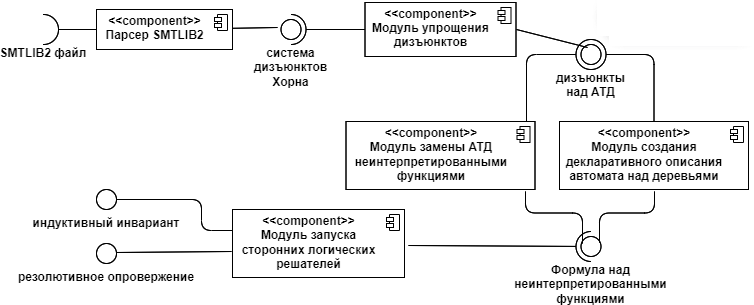
\includegraphics[width=\textwidth]{resources/arch.png}
\caption{Хорн-решатель \theringen{}: \url{https://github.com/Columpio/RInGen}}
% \label{fig:ringen-arch}
\end{figure}
\end{frame}

\begin{frame}{Сравнение Хорн-решателей с поддержкой АТД}
\begin{table}
\centering\footnotesize
% \caption{Сравнение Хорн-решателей с поддержкой АТД}\label{tab:hornSolvers}%
\begin{tabular}{| m{38mm} || x{18mm} | x{18mm} | x{18mm} | x{23mm} |}
% \hline
\hline
Инструмент & Класс\quad\ \ \  инвариантов & Метод & Возвращает инвариант & Полностью автоматический\\\hline\hline
\spacer{} & \elemclass{} & \pdr{} & Да & Да\\
\racer{} & \catelemclass{} & \pdr{} & Нет & Нет\\
\eldarica{} & \sizeelemclass{} & \cegar{} & Да & Да\\
\vericat{} & -- & Трансф. & Нет & Да\\
\hoice{} & \elemclass{} & \ice{} & Да & Да\\
\rchc{}  & \syncRegFlatClass{} & \ice{} & Да & Да\\\hline
\ringen{\cvc} & \regclass{} & Трансф. + \fmf{} & Да & Да\\
\ringen{\vampire} & -- & Трансф. + \satur{} & Нет & Да\\
\ringenSync{} & \syncRegFullClass{} & Трансф. + \fmf{} & Да & Да\\
\ringenCICI{\cvc} & \regelemclass{} & \ourCEGAR{} & Да & Да\\
\ringenCICI{\vampire} & -- & \ourCEGAR{} & Нет & Да\\
\hline
% \hline
\end{tabular}
\end{table}
\end{frame}

\begin{frame}{Эксперименты}
\vspace*{-10pt}
\begin{columns}
\begin{column}{.42\textwidth}
\begin{table}
% \caption{Результаты экспериментов. <<SAT>> обозначает, что система безопасна (есть индуктивный инвариант), <<UNSAT>> обозначает, что система небезопасна.}
% \label{table:eval-all}
\scriptsize
\centering
\begin{tabular}{ |l||c|c| }
\hline
Инструмент & SAT & UNSAT\\\hline\hline
\racer{} & 26 & 22\\
\eldarica{} & 46 & 12\\
\vericat{} & 16 & 10\\
\cvcind{} & 0 & 13\\
\hline
\ringen{\cvc{}} & 25 & 21\\
\ringen{\vampire{}} & 135 & 46\\
\ringenSync{} & 43 & 21\\
\ringenCICI{\cvc{}} & 117 & 19\\
\ringenCICI{\vampire{}} & 189 & 28\\
\hline
\end{tabular}
\end{table}
\end{column}
\begin{column}{.5\textwidth}
\pgfplotstableread[col sep = comma]{resources/experiments1.csv}\all
\begin{figure}[h]
\begin{center}
\begin{tikzpicture}[scale=0.55]
\begin{axis}[xmode=log, ymode=log, legend pos= north west, xlabel={Время работы \ringen{\cvc{}}, мс}, xlabel style = {align=center,font=\footnotesize}, ylabel style = {align=center,font=\footnotesize}, ylabel={Время работы {\color{red}\racer{}}, {\color{blue}\eldarica{}},\\{\color{brown}\cvcind{}} и {\color{cyan}\verimap{}}, мс}]
% \begin{axis}[xmode=log, ymode=log, legend pos= north west, xlabel={ Regular model construction by \theringen{}}, ylabel style = {align=center}, ylabel={Elementary model construction by \\{\color{red}\textsc{Spacer}}, {\color{blue}\eldarica{}} and {\color{brown}\cvcind{}}}]
    \addplot[dashed,no marks,very thin] coordinates {(10,10) (600000,600000)};
    \addplot [dashed, no marks, thin] coordinates {(10,10) (600000,600000)};
    \addplot [dashed, no marks, thin] coordinates {(10,300000) (300000,300000)};
    \addplot [dashed, no marks, thin] coordinates {(300000, 10) (300000,300000)};
    \addplot [dashed, no marks, thin] coordinates {(10, 600000) (600000,600000)};
    \addplot [dashed, no marks, thin] coordinates {(600000, 10) (600000,600000)};

    \addplot  [only marks,  mark=triangle, color=blue, mark size=3pt] table [x={CVC4Finite}, y={Eldarica}] {\all};
    \addplot  [only marks,  mark=o, color=red,  mark size=3pt] table [x={CVC4Finite}, y={Z3}] {\all};
    \addplot  [only marks,  mark=x, color=brown, mark size=3pt] table [x={CVC4Finite}, y={CVC4Ind}] {\all};
    \addplot  [only marks,  mark=square, color=cyan, mark size=3pt] table [x={CVC4Finite}, y={VeriMAP-iddt}] {\all};
\end{axis}

\end{tikzpicture}
    % \caption{Сравнение производительности инструментов. Каждая точка на графике представляет пару длительностей выполнения.}
% \label{fig:toolplotOne}
\end{center}
\end{figure}
\end{column}
\end{columns}
\vspace*{-5pt}
\begin{figure}
\toolplotTwo{\cvc{}}{resources/toolplot_cvc.csv}
~
\toolplotTwo{\vampire{}}{resources/toolplot_vampire.csv}
% \caption{Сравнение времени работы инструментов}
% \label{fig:toolplot}
\end{figure}
\end{frame}


\begin{frame}{Результаты}
\begin{enumerate}
\item Предложен метод вывода регулярных инвариантов при помощи поиска конечных моделей и доказана его корректность
\item Предложен метод вывода синхронных регулярных инвариантов при помощи поиска конечных моделей и доказана его корректность
\item Предложен новый класс инвариантов, основанный на булевой комбинации элементарных и регулярных инвариантов
\item Предложен метод совместного вывода инвариантов в этом классе посредством вывода инвариантов в подклассах и доказана его корректность
\item Проведено теоретическое сравнение рассмотренных классов инвариантов, доказаны леммы о накачке для языков первого порядка
\item Выполнена пилотная реализация предложенных методов на языке \fsharp{} в рамках инструмента \theringen{}\\Разработанный инструмент решил из бенчмарка <<Tons of Inductive Problems>> в 3.74 раза больше задач, чем наилучший из существующих инструментов
\end{enumerate}
\end{frame}

\begin{frame}{Соответствие результатов паспорту специальности 2.3.5}

Результаты соответствуют направлению исследования  № 1
\begin{itemize}
\item Модели, \textbf{методы и алгоритмы} проектирования, анализа, трансформации, \textbf{верификации} и тестирования \textbf{программ} и программных систем
\end{itemize}
из паспорта специальности.
\end{frame}

\begin{framesection}{Научная новизна}
\begin{enumerate}
\item Впервые предложен класс инвариантов, основанный на булевой комбинации элементарных и регулярных инвариантов
\item Впервые предложен алгоритм вывода инвариантов для программ с АТД, основанный на поиске конечных моделей
\item Предложен новый алгоритм совместного вывода инвариантов в комбинации классов инвариантов на базе методов вывода инвариантов в подклассах
\item Впервые введены и доказаны леммы о <<накачке>> для языков первого порядка в сигнатуре теории АТД
\end{enumerate}
\end{framesection}

\section{Публикации и выступления}
\begin{frame}{Публикации по теме диссертации}
% \begin{table}
% \centering
% \begin{tabular}{p{.3\textwidth}|p{.7\textwidth}}
% \citep{kostyukov2019auto} & автор выполнил реализацию сведения поиска индуктивных инвариантов функций над сложными структурами данных к решению систем дизъюнктов Хорна, а также спроектировал эксперименты с различными существующими Хорн-решателями\\
% % ; соавторы предложили саму идею и проработали её теоретические аспекты
% \citep{10.1145/3453483.3454055} & автор провёл теоретическое сопоставление классов индуктивных инвариантов, предложил и доказал леммы о <<накачке>> для языков первого порядка над АТД, реализовал предлагаемый подход, поставил эксперименты\\
% % ; соавторы участвовали в обсуждении основных идей статьи, выполнили обзор существующих решений
% \citep{LPAR2023:Collaborative_Inference_of_Combined} & автор предложил и формально обосновал коллаборационный подход к выводу инвариантов, реализовал прототип и поставил эксперименты\\
% % ; соавторы участвовали в обсуждении презентации идей статьи и выполнили обзор существующих решений
% \citep{miso2022gen} & вклад автора заключается в формальном описании теории вычисления предусловий программ со сложными структурами данных
% % ; соавторы участвовали в обсуждении основных идей и реализовали подход
%     \end{tabular}
% \end{table}
\footnotesize
\bibliographystyle{ugost2008ls}
\bibliography{bibliography.bib}
\nocite{kostyukov2019auto}
\nocite{10.1145/3453483.3454055}
\nocite{LPAR2023:Collaborative_Inference_of_Combined}
\nocite{miso2022gen}
% \begin{enumerate}
% \item \citee{kostyukov2019auto}
% \item \citee{10.1145/3453483.3454055}
% \item \citee{LPAR2023:Collaborative_Inference_of_Combined}
% \item \citee{miso2022gen}
% \end{enumerate}
\end{frame}

\begin{frame}{Выступления по теме диссертации}
\begin{itemize}
\item Международный семинар HCVS 2021 (28 марта 2021, Люксембург)
\item Семинар компании Huawei (18-19 ноября 2021, Санкт-Петербург)
\item Ежегодный внутренней семинар JetBrains Research (18 декабря 2021, Санкт-Петербург)
\item Конференция PLDI 2021 (23-25 июня 2021, Канада)
\item Внутренний семинар Венского технического университета (3 июня 2022, Австрия)
\item Конференция LPAR 2023 (4-9 июня 2023, Колумбия)
\end{itemize}

Разработанный инструмент в 2021 и 2022 годах занял, соответственно, 2 и 1 место на АТД секции международных соревнований \chccomp{}.
\end{frame}

% Extra
\begin{frame}{Сравнение Хорн-решателей с поддержкой АТД}
\begin{table}
\centering\footnotesize
% \caption{Сравнение Хорн-решателей с поддержкой АТД}\label{tab:hornSolvers}%
\begin{tabular}{| m{38mm} || x{18mm} | x{18mm} | x{18mm} | x{23mm} |}
% \hline
\hline
Инструмент & Класс\quad\ \ \  инвариантов & Метод & Возвращает инвариант & Полностью автоматический\\\hline\hline
\spacer{} & \elemclass{} & \pdr{} & Да & Да\\
\racer{} & \catelemclass{} & \pdr{} & Нет & Нет\\
\eldarica{} & \sizeelemclass{} & \cegar{} & Да & Да\\
\vericat{} & -- & Трансф. & Нет & Да\\
\hoice{} & \elemclass{} & \ice{} & Да & Да\\
\rchc{}  & \syncRegFlatClass{} & \ice{} & Да & Да\\\hline
\ringen{\cvc} & \regclass{} & Трансф. + \fmf{} & Да & Да\\
\ringen{\vampire} & -- & Трансф. + \satur{} & Нет & Да\\
\ringenSync{} & \syncRegFullClass{} & Трансф. + \fmf{} & Да & Да\\
\ringenCICI{\cvc} & \regelemclass{} & \ourCEGAR{} & Да & Да\\
\ringenCICI{\vampire} & -- & \ourCEGAR{} & Нет & Да\\
\hline
% \hline
\end{tabular}
\end{table}
\end{frame}

\end{document}


\begin{frame}{ATP-based CHC solving\footnote{Details in our PLDI'21 paper:\\\quad``Beyond the elementary representations of program invariants over algebraic data types''}}
\begin{itemize}
    \item<+-> Can we infer \attention{not FOL-based} inductive invariants by employing ATPs?
    \item<+-> Note that a Herbrand model is \attention{almost} a model of the ADT theory
    \item<+-> Yet it \attention{lacks} testers, selectors, and \attention{treats} disequality constraints \attention{differently}
    \item<+-> By syntactic manipulations, CHCs over ADTs can be reduced to the \attention{\textit{free theory}}$^1$
    \vspace*{4mm}\begin{itemize}
        \item i.e., pure first-order logic without any theory axioms
    \end{itemize}
    \item<+-> After that, \attention{any} automated theorem prover can be \attention{soundly used}
\end{itemize}
\end{frame}

\section{Collaborative Inference of Combined Invariants}

\begin{frame}{Implementation}
    \centering\begin{tikzpicture}[font=\Large]
        \node (pic) {\includegraphics[width=.5\textwidth]{resources/spacer_and_vampire.png}};
        \node at (-2.2, -3) {\textsc{Z3 Spacer}};
        \node at (2.2, -3) {\textsc{Vampire}};
        \calloutquote[position={(-2.1,-0.8)},bubblePosition={(1.9,3.3)},callout pointer width=.4cm,fill=focusRed!70,rounded corners]{residual system}
        \calloutquote[position={(1.9,-1.6)},bubblePosition={(-1.9,3.3)},callout pointer width=.4cm,fill=focusBlue!50,rounded corners]{part of invariant}
    \end{tikzpicture}
\end{frame}

\begin{frame}{Experiments: solved systems}
    \centering
    \Large
\begin{table}[h]
    % \small
    % \begin{tabular}{ |c|c|r|c|c|c|c|c|  }
    \begin{tabular}{ |r|c|c|c|c|c|  }
     \hline
     % \multirow{2}{*}{Benchmark} & \multirow{2}{*}{\#} &
     \multirow{2}{*}{Answer} & \multicolumn{2}{c|}{\ringen{}} & \multirow{2}{*}{\spacer{}} & \multicolumn{2}{c|}{\collab{}}\\
     % \cline{4-5}\cline{7-8}
     \cline{2-3}\cline{5-6}
     % &&
     & \cvc{} & \vampire{} && \cvc{} & \vampire{}\\\hline

     % \multirow{2}{*}{\emph{TIP}} & \multirow{2}{*}{454} &
     SAT                   & 25    & 135    & 20   & 117  & \textbf{189}  \\
     % && Unique SAT          & 8     & 48     &  6    &  19   &  21 \\
     % &&
     UNSAT               & 21    & \textbf{46}     & 15    & 19    & 28\\
     % && Unique UNSAT        & 0     & 18     & 2     & 0     & 0\\
     \hline
    \end{tabular}

    % \caption{Time limit: 600 seconds}
\end{table}
Time limit: 600 seconds

% \onslide<2->{
\begin{align*}
  \collab(\spacer{}, \vampire{}) &> \spacer{} \parallel \vampire{}\\
  \collab(\spacer{}, \cvc{}) &> \spacer{} \parallel \cvc{}
\end{align*}
% }
\end{frame}

\begin{frame}{Highlights}
\large
\begin{itemize}
\item<+-> Many practical tasks reduce to CHC solving
\item<+-> CHC solvers build infinite models modulo theories
\item<+-> CHC solvers compute approximations instead of least fixed points
\item<+-> ATPs can be used as CHC solvers for ADTs via simple trick
\item<+-> CHC solvers and ATPs can collaborate instead of competing
\item<+-> Collaboration of CHC solvers and ATPs is strictly stronger than parallel
\end{itemize}

\onslide<7->{\vspace*{10mm}
\centering\Large Thank you! Questions?}
\end{frame}

\appendix

\begin{frame}{Experiments: solving time}
\centering
\Large
\begin{tikzpicture}[scale=.8]
\begin{scope}[shift={(-5,0)}]
\toolplot{\cvc{}}{resources/toolplot_cvc.csv}
\end{scope}
\begin{scope}[shift={(4,0)}]
\toolplot{\vampire{}}{resources/toolplot_vampire.csv}
\end{scope}
\end{tikzpicture}

Runtimes in milliseconds
\end{frame}

\begin{frame}{CHC solvers and CHC Competition 2022}
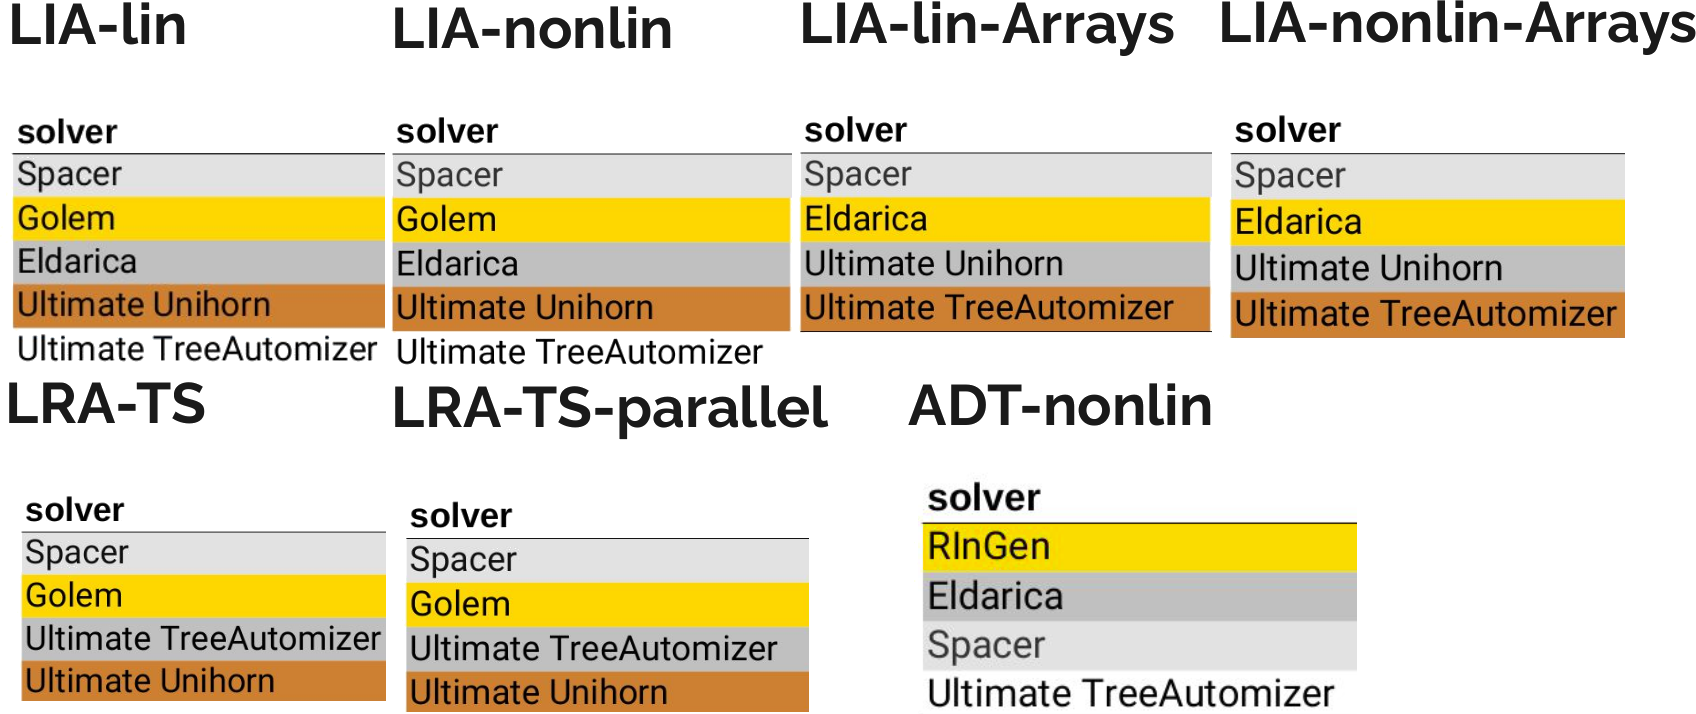
\includegraphics[width=\textwidth]{resources/chccomp_all.png}
\begin{tikzpicture}[remember picture,overlay]
\begin{scope}[shift={(-0.5,-0.3)}]
% \onslide<2->{\calloutquote[width=3.7cm,position={(-1.08,-0.55)},bubblePosition={(2.8,6.15)},callout pointer width=.5cm,fill=blue!30,rounded corners]{IC3/PDR engine in \textsc{Z3}}
% \calloutquote[width=2.5cm,position={(-1.5,-1)},bubblePosition={(6.4,6.15)},callout pointer width=.5cm,fill=green!40,rounded corners]{Portfolio solver}
% \calloutquote[width=5.6cm,position={(-2.,-1)},bubblePosition={(11,6.15)},callout pointer width=.7cm,fill=yellow!50,rounded corners]{CEGAR with predicate abstraction}
% }
\onslide<2->{
\draw[draw=nicegreen!70,ultra thick] (7.8, 0) rectangle ++(4.2, 3.8);
\calloutquote[width=2.4cm,position={(-1.1,-0.3)},bubblePosition={(12,2.7)},callout pointer width=.4cm,fill=nicegreen!70,rounded corners]{\Large\centering Our journey begins here}}
\end{scope}
\end{tikzpicture}
\end{frame}

\begin{frame}{How RInGen works}
% \centering\begin{tikzpicture}[remember picture,overlay]
% \node[draw,fill=blue!30,opacity=0.8,rounded rectangle,rotate=0,align=center,font=\small] at (0,-2) {* Details in our PLDI'21 paper\\``Beyond the elementary representations of program invariants over algebraic data types''};
% \end{tikzpicture}
% \begin{tikzpicture}[draw,opacity=0.95,rounded rectangle]
% \node[fill=blue!30] at (0, 0) {}
% \end{tikzpicture}
\begin{tikzpicture}
\node[draw,fill=blue!30,opacity=0.95,rounded rectangle] at (0, 0) {Can we infer not FOL-based inductive invariants by employing ATPs?};
\onslide<2->{\node[draw,fill=green!40,opacity=0.95,rounded rectangle] at (2.5, -0.7) {Because obtained model may violate ADT theory axioms};}
\onslide<3->{\node[draw,fill=green!40,opacity=0.95,rounded rectangle] at (1.85, -1.4) {The \textbf{only} reason why Herbrand model does not fit are \textbf{equalities}};}
\end{tikzpicture}
\onslide<4->{
\centering $\Rightarrow$ Eliminate equalities by adding extra CHCs, e.g.:
\begin{align*}
    \bot&\leftarrow \neg(Z = S(Z))\\
    \text{should}&\text{ become}\\
    \bot&\leftarrow diseq_{Nat}(Z, S(Z))\\
    diseq_{Nat}(Z, S(x))&\leftarrow \top\\
    diseq_{Nat}(S(x), Z)&\leftarrow \top\\
    diseq_{Nat}(S(x), S(y))&\leftarrow diseq_{Nat}(x, y)
\end{align*}}
\begin{tikzpicture}[remember picture,overlay]
\onslide<5->{\node[draw,fill=green!40,opacity=0.95,rounded rectangle] at (2, 0.3) {The obtained CHC system can be soundly thrown into ATP};}
\onslide<6>{\node[overlay,draw,fill=blue!30,opacity=0.95,rounded rectangle,minimum height=1.5cm,minimum width=6cm, rotate=15,align=center] at (0,3) {{\huge Details in our PLDI'21 paper}\\{``Beyond the elementary representations of program invariants over algebraic data types''}};}
\end{tikzpicture}
\end{frame}

\whenFullCompile{\input{RInGenHowTo}}

\begin{frame}{ATP-based CHC solving}
\begin{tikzpicture}
\onslide<1->{\node[draw,fill=blue!30,opacity=0.95,rounded rectangle] at (-2, 0) {What kind of inductive invariants can be inferred this way?};}
\onslide<2->{\node[draw,fill=green!40,opacity=0.95,rounded rectangle,align=center] at (2.3, -0.9) {Depends on ATP backend: e.g., if it is a finite-model finder, then\\
it infers \textbf{regular} inductive invariants based on tree automata};}
\end{tikzpicture}

\onslide<3->{
For $even$ example it automatically infers the following inductive invariant:
$$ \invariant \equiv \mathcal{H}\left\{ even \mapsto \mathcal{L}\left(\mathcal{A}\right) \right\} \equiv \mathcal{H}\left\{ even \mapsto\left\{ S^{2n}(Z) \mid n \geq 0 \right\}\right\}$$
based on the tree automaton
$$ \mathcal{A} = \theAutomatoN{s_0, s_1}{\{Z, S\}}{s_0}{\Delta} $$
\vspace*{-10mm}\exampleEven{}}
\begin{tikzpicture}
\onslide<4->{\node[draw,fill=green!40,opacity=0.95,rounded rectangle,align=center] at (0, 0) {\Large The power of the technique is that \textbf{any ATP} can be soundly used};}
\end{tikzpicture}
\end{frame}

\end{document}

% \begin{frame}{Our success on Horn solving competition: \ringen{} with Vampire backend}
% 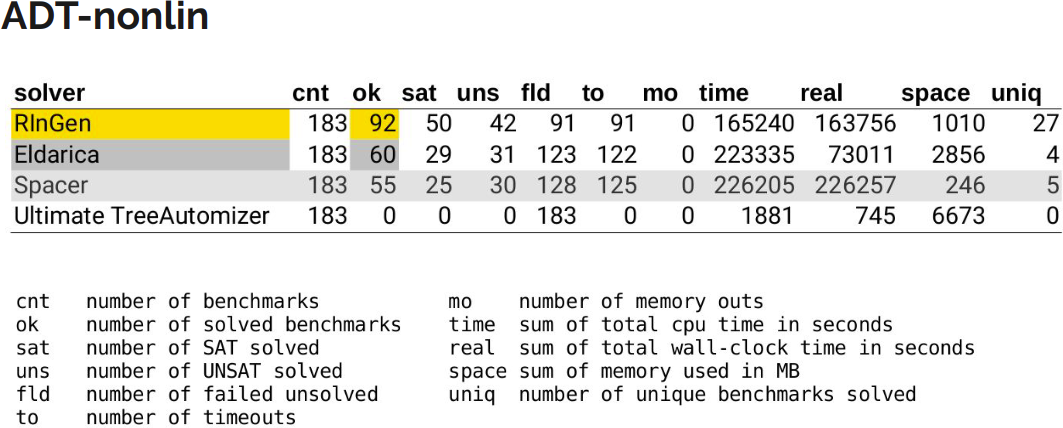
\includegraphics[width=\textwidth]{resources/chccompres.png}
% \begin{tikzpicture}[remember picture,overlay]
% \onslide<2->{\calloutquote[width=3cm,position={(-1,-0.02)},bubblePosition={(5.5,6.4)},fill=red!30,rounded corners]{ADT track on CHC-COMP 2022}}
% \onslide<3->{\calloutquote[width=3.2cm,position={(-1,1.39)},bubblePosition={(2.5,2)},fill=green!30,rounded corners]{CHC-COMP winner for last 4 years}}
% \onslide<4->{
% \draw[draw=blue!30,ultra thick] (5,3) rectangle ++(2.45,2.6);
% \draw[draw=blue!30,ultra thick] (9.97,3) rectangle ++(1.45,2.6);
% \calloutquote[width=4.4cm,position={(-2,-0.55)},bubblePosition={(10,6.4)},callout pointer width=.5cm,fill=blue!30,rounded corners]{win by sat, unsat and time}
% \calloutquote[width=4.4cm,position={(.5,-0.55)},bubblePosition={(10,6.4)},callout pointer width=.3cm,fill=blue!30,rounded corners]{win by sat, unsat and time}
% }
% \end{tikzpicture}
% \end{frame}



% \begin{frame}{Useful links}
% \begin{itemize}
% \item State-of-art Horn solver \spacer{}/\textsc{Spacer}: \url{https://github.com/z3prover/z3}
% \item Our Horn solver \ringen{}: \url{https://github.com/Columpio/RInGen}
% \item Our PLDI paper on \ringen{}: \url{https://arxiv.org/abs/2104.04463}
% \item Our Vampire fork: \url{https://github.com/Columpio/Vampire/tree/chc-comp22}
% \item Demo files for these slides: \url{https://gitlab.com/Columpio/demos}
% \item CHC-COMP results: \href{https://chc-comp.github.io/CHC-COMP2022_presentation.pdf}{\detokenize{chc-comp.github.io/CHC-COMP2022_presentation.pdf}}
% \end{itemize}
% \end{frame}